% Options for packages loaded elsewhere
\PassOptionsToPackage{unicode}{hyperref}
\PassOptionsToPackage{hyphens}{url}
\PassOptionsToPackage{dvipsnames,svgnames,x11names}{xcolor}
%
\documentclass[
  10pt,
]{article}
\usepackage{amsmath,amssymb}
\usepackage{iftex}
\ifPDFTeX
  \usepackage[T1]{fontenc}
  \usepackage[utf8]{inputenc}
  \usepackage{textcomp} % provide euro and other symbols
\else % if luatex or xetex
  \usepackage{unicode-math} % this also loads fontspec
  \defaultfontfeatures{Scale=MatchLowercase}
  \defaultfontfeatures[\rmfamily]{Ligatures=TeX,Scale=1}
\fi
\usepackage{lmodern}
\ifPDFTeX\else
  % xetex/luatex font selection
\fi
% Use upquote if available, for straight quotes in verbatim environments
\IfFileExists{upquote.sty}{\usepackage{upquote}}{}
\IfFileExists{microtype.sty}{% use microtype if available
  \usepackage[]{microtype}
  \UseMicrotypeSet[protrusion]{basicmath} % disable protrusion for tt fonts
}{}
\makeatletter
\@ifundefined{KOMAClassName}{% if non-KOMA class
  \IfFileExists{parskip.sty}{%
    \usepackage{parskip}
  }{% else
    \setlength{\parindent}{0pt}
    \setlength{\parskip}{6pt plus 2pt minus 1pt}}
}{% if KOMA class
  \KOMAoptions{parskip=half}}
\makeatother
\usepackage{xcolor}
\usepackage[left=2cm, right=2cm, top=2cm, bottom=3cm, footskip = .5cm]{geometry}
\usepackage{longtable,booktabs,array}
\usepackage{calc} % for calculating minipage widths
% Correct order of tables after \paragraph or \subparagraph
\usepackage{etoolbox}
\makeatletter
\patchcmd\longtable{\par}{\if@noskipsec\mbox{}\fi\par}{}{}
\makeatother
% Allow footnotes in longtable head/foot
\IfFileExists{footnotehyper.sty}{\usepackage{footnotehyper}}{\usepackage{footnote}}
\makesavenoteenv{longtable}
\usepackage{graphicx}
\makeatletter
\def\maxwidth{\ifdim\Gin@nat@width>\linewidth\linewidth\else\Gin@nat@width\fi}
\def\maxheight{\ifdim\Gin@nat@height>\textheight\textheight\else\Gin@nat@height\fi}
\makeatother
% Scale images if necessary, so that they will not overflow the page
% margins by default, and it is still possible to overwrite the defaults
% using explicit options in \includegraphics[width, height, ...]{}
\setkeys{Gin}{width=\maxwidth,height=\maxheight,keepaspectratio}
% Set default figure placement to htbp
\makeatletter
\def\fps@figure{htbp}
\makeatother
\setlength{\emergencystretch}{3em} % prevent overfull lines
\providecommand{\tightlist}{%
  \setlength{\itemsep}{0pt}\setlength{\parskip}{0pt}}
\setcounter{secnumdepth}{-\maxdimen} % remove section numbering
% Set up the fonts
\usepackage[urw-palatino]{mathdesign}
\usepackage[T1]{fontenc}

% Add accessibility support from http://www.richschwinn.com/accessibility
\RequirePackage{accsupp}
\RequirePackage{pdfcomment}
\newcommand{\AccTool}[2]{\BeginAccSupp{method=pdfstringdef,unicode,Alt={{#1}}}\pdftooltip{{#2}}{{#1}}\EndAccSupp{}}

% Set the language for 508
\hypersetup{
  pdftitle = {title},
  pdflang = en-US}


% Set up the headers and footers
\usepackage{graphicx}
\usepackage{fancyhdr}
\usepackage{ifthen}
%\usepackage{everypage-1x}
\usepackage{float}
%\usepackage{subfig}
%\usepackage{subcaption}

% Avoid struggling over figure and table float in Rmarkdown
\let\origfigure\figure
\let\endorigfigure\endfigure
\renewenvironment{figure}[1][2] {
    \expandafter\origfigure\expandafter[H]
} {
    \endorigfigure
}

\let\origtable\table
\let\endorigtable\endtable
\renewenvironment{table}[1][2] {
    \expandafter\origtable\expandafter[H]
} {
    \endorigtable
}

% First page has the large title and NOAA logo
\pagestyle{fancy}
\fancyhf{}
\setlength\headheight{40pt}
\fancyheadoffset[L]{0.5cm}
\cfoot{\thepage}

\fancyheadinit{%
   \ifthenelse{\value{page}=5}%
      {\fancyhead[R]{
\includegraphics[width=40pt]{images/NOAA_logo.png} \\ \textsf{\emph{January 27, 2025}}}
       \fancyhead[L]{\textsf{\LARGE DRAFT State of the Ecosystem 2025: New England}}
      }%
      {\fancyhead[R]{}
       \fancyhead[L]{\textsf{\emph{DRAFT State of the Ecosystem 2025: New England}}}
      }
}



\renewcommand{\headrulewidth}{0.4pt}
\renewcommand{\footrulewidth}{0pt}

% Make caption fonts a bit smaller
\usepackage[font={small}]{caption}


% Change section labels to san serif
\usepackage{sectsty}
\allsectionsfont{\normalfont\sffamily\bfseries}
\usepackage{multirow}
\usepackage{multicol}
\usepackage{colortbl}
\usepackage{hhline}
\newlength\Oldarrayrulewidth
\newlength\Oldtabcolsep
\usepackage{longtable}
\usepackage{array}
\usepackage{hyperref}
\usepackage{float}
\usepackage{wrapfig}
\ifLuaTeX
  \usepackage{selnolig}  % disable illegal ligatures
\fi
\IfFileExists{bookmark.sty}{\usepackage{bookmark}}{\usepackage{hyperref}}
\IfFileExists{xurl.sty}{\usepackage{xurl}}{} % add URL line breaks if available
\urlstyle{same}
\hypersetup{
  colorlinks=true,
  linkcolor={Maroon},
  filecolor={Maroon},
  citecolor={Blue},
  urlcolor={blue},
  pdfcreator={LaTeX via pandoc}}

\author{}
\date{\vspace{-2.5em}}

\begin{document}

\setcounter{page}{5}
\thispagestyle{fancy}

\hypertarget{introduction}{%
\section{Introduction}\label{introduction}}

\hypertarget{about-this-report}{%
\subsection{About This Report}\label{about-this-report}}

This report is for the New England Fishery Management Council (NEFMC). The purpose of this report is to synthesize ecosystem information to allow the NEFMC to better meet fishery management objectives. The major messages of the report are synthesized on pages 1-3, with highlights of 2024 ecosystem events on page 4. The information in this report is organized into two main sections; \protect\hyperlink{performance-relative-to-fishery-management-objectives}{performance measured against ecosystem-level management objectives} (Table \ref{tab:management-objectives}), and potential \protect\hyperlink{risks-to-meeting-fishery-management-objectives}{risks to meeting fishery management objectives} (\protect\hyperlink{climate-and-ecosystem-change}{climate change} and \protect\hyperlink{other-ocean-uses-offshore-wind}{other ocean uses}). A final new section introduced as last year's highlights \protect\hyperlink{highlights}{notable 2024 ecosystem observations}.

\hypertarget{report-structure}{%
\subsection{Report structure}\label{report-structure}}

A glossary of terms\footnote{\url{https://noaa-edab.github.io/tech-doc/glossary.html}}, detailed technical methods documentation\footnote{\url{https://NOAA-EDAB.github.io/tech-doc}} and indicator data\footnote{\url{https://github.com/NOAA-EDAB/ecodata}}, and detailed indicator descriptions\footnote{\url{https://noaa-edab.github.io/catalog/index.html}} are available online. We recommend new readers first review the details of standard figure formatting (Fig. \ref{fig:docformat}a), categorization of fish and invertebrate species into feeding guilds (Table \ref{tab:species-groupings}), and definitions of ecological production units (EPUs, including the Gulf of Maine (GOM) and Georges Bank (GB); Fig. \ref{fig:docformat}b) provided at the end of the document.

The two main sections contain subsections for each management objective or potential risk. Within each subsection, we first review indicator trends, and the status of the most recent data year relative to a threshold (if available) or relative to the long-term average. Second, we synthesize results of other indicators and information to outline potential implications for management (i.e., connecting indicator status to management and why an indicator is important). For example, if there are multiple drivers related to an indicator trend, we examine which drivers may be more or less supported by current information, and which, if any, are affected by management actions? Similarly, we examine which risk indicators warrant continued monitoring to evaluate whether regime shifts or ecosystem reorganization are likely? We emphasize that these implications are intended to represent testable hypotheses at present, rather than ``answers,'' because the science behind these indicators and syntheses continues to develop.

\global\setlength{\Oldarrayrulewidth}{\arrayrulewidth}

\global\setlength{\Oldtabcolsep}{\tabcolsep}

\setlength{\tabcolsep}{0pt}

\renewcommand*{\arraystretch}{1}



\providecommand{\ascline}[3]{\noalign{\global\arrayrulewidth #1}\arrayrulecolor[HTML]{#2}\cline{#3}}

\begin{longtable}[c]{|p{1.77in}|p{4.09in}}

\caption{Ecosystem-scale\ fishery\ management\ objectives\ in\ the\ Mid-Atlantic\ Bight}\label{tab:management-objectives}\\

\ascline{1.5pt}{666666}{1-2}

\multicolumn{1}{>{\raggedright}m{\dimexpr 1.77in+0\tabcolsep}}{\textcolor[HTML]{000000}{\fontsize{9}{9}\selectfont{Objective\ categories}}} & \multicolumn{1}{>{\raggedright}m{\dimexpr 4.09in+0\tabcolsep}}{\textcolor[HTML]{000000}{\fontsize{9}{9}\selectfont{Indicators\ reported}}} \\

\ascline{1.5pt}{666666}{1-2}\endfirsthead \caption[]{Ecosystem-scale\ fishery\ management\ objectives\ in\ the\ Mid-Atlantic\ Bight}\label{tab:management-objectives}\\

\ascline{1.5pt}{666666}{1-2}

\multicolumn{1}{>{\raggedright}m{\dimexpr 1.77in+0\tabcolsep}}{\textcolor[HTML]{000000}{\fontsize{9}{9}\selectfont{Objective\ categories}}} & \multicolumn{1}{>{\raggedright}m{\dimexpr 4.09in+0\tabcolsep}}{\textcolor[HTML]{000000}{\fontsize{9}{9}\selectfont{Indicators\ reported}}} \\

\ascline{1.5pt}{666666}{1-2}\endhead



\multicolumn{2}{>{\raggedright}m{\dimexpr 5.86in+2\tabcolsep}}{\textcolor[HTML]{000000}{\fontsize{9}{9}\selectfont{\textbf{Objectives:\ Provisioning\ and\ Cultural\ Services}}}} \\





\multicolumn{1}{>{\raggedright}m{\dimexpr 1.77in+0\tabcolsep}}{\textcolor[HTML]{000000}{\fontsize{9}{9}\selectfont{Seafood\ Production}}} & \multicolumn{1}{>{\raggedright}m{\dimexpr 4.09in+0\tabcolsep}}{\textcolor[HTML]{000000}{\fontsize{9}{9}\selectfont{Landings;\ commercial\ total\ and\ by\ feeding\ guild;\ recreational\ harvest}}} \\





\multicolumn{1}{>{\raggedright}m{\dimexpr 1.77in+0\tabcolsep}}{\textcolor[HTML]{000000}{\fontsize{9}{9}\selectfont{Commercial\ Profits}}} & \multicolumn{1}{>{\raggedright}m{\dimexpr 4.09in+0\tabcolsep}}{\textcolor[HTML]{000000}{\fontsize{9}{9}\selectfont{Revenue\ decomposed\ to\ price\ and\ volume}}} \\





\multicolumn{1}{>{\raggedright}m{\dimexpr 1.77in+0\tabcolsep}}{\textcolor[HTML]{000000}{\fontsize{9}{9}\selectfont{Recreational\ Opportunities}}} & \multicolumn{1}{>{\raggedright}m{\dimexpr 4.09in+0\tabcolsep}}{\textcolor[HTML]{000000}{\fontsize{9}{9}\selectfont{Angler\ trips;\ recreational\ fleet\ diversity}}} \\





\multicolumn{1}{>{\raggedright}m{\dimexpr 1.77in+0\tabcolsep}}{\textcolor[HTML]{000000}{\fontsize{9}{9}\selectfont{Stability}}} & \multicolumn{1}{>{\raggedright}m{\dimexpr 4.09in+0\tabcolsep}}{\textcolor[HTML]{000000}{\fontsize{9}{9}\selectfont{Diversity\ indices\ (fishery\ and\ ecosystem)}}} \\





\multicolumn{1}{>{\raggedright}m{\dimexpr 1.77in+0\tabcolsep}}{\textcolor[HTML]{000000}{\fontsize{9}{9}\selectfont{Social\ \&\ Cultural}}} & \multicolumn{1}{>{\raggedright}m{\dimexpr 4.09in+0\tabcolsep}}{\textcolor[HTML]{000000}{\fontsize{9}{9}\selectfont{Community\ fishing\ engagement\ and\ social\ vulnerability\ status}}} \\





\multicolumn{1}{>{\raggedright}m{\dimexpr 1.77in+0\tabcolsep}}{\textcolor[HTML]{000000}{\fontsize{9}{9}\selectfont{Protected\ Species}}} & \multicolumn{1}{>{\raggedright}m{\dimexpr 4.09in+0\tabcolsep}}{\textcolor[HTML]{000000}{\fontsize{9}{9}\selectfont{Bycatch;\ population\ (adult\ and\ juvenile)\ numbers;\ mortalities}}} \\





\multicolumn{2}{>{\raggedright}m{\dimexpr 5.86in+2\tabcolsep}}{\textcolor[HTML]{000000}{\fontsize{9}{9}\selectfont{\textbf{Potential\ Drivers:\ Supporting\ and\ Regulating\ Services}}}} \\





\multicolumn{1}{>{\raggedright}m{\dimexpr 1.77in+0\tabcolsep}}{\textcolor[HTML]{000000}{\fontsize{9}{9}\selectfont{Management}}} & \multicolumn{1}{>{\raggedright}m{\dimexpr 4.09in+0\tabcolsep}}{\textcolor[HTML]{000000}{\fontsize{9}{9}\selectfont{Stock\ status;\ catch\ compared\ with\ catch\ limits}}} \\





\multicolumn{1}{>{\raggedright}m{\dimexpr 1.77in+0\tabcolsep}}{\textcolor[HTML]{000000}{\fontsize{9}{9}\selectfont{Biomass}}} & \multicolumn{1}{>{\raggedright}m{\dimexpr 4.09in+0\tabcolsep}}{\textcolor[HTML]{000000}{\fontsize{9}{9}\selectfont{Biomass\ or\ abundance\ by\ feeding\ guild\ from\ surveys}}} \\

\ascline{1.5pt}{666666}{1-2}



\end{longtable}



\arrayrulecolor[HTML]{000000}

\global\setlength{\arrayrulewidth}{\Oldarrayrulewidth}

\global\setlength{\tabcolsep}{\Oldtabcolsep}

\renewcommand*{\arraystretch}{1}

\global\setlength{\Oldarrayrulewidth}{\arrayrulewidth}

\global\setlength{\Oldtabcolsep}{\tabcolsep}

\setlength{\tabcolsep}{0pt}

\renewcommand*{\arraystretch}{1}



\providecommand{\ascline}[3]{\noalign{\global\arrayrulewidth #1}\arrayrulecolor[HTML]{#2}\cline{#3}}

\begin{longtable}[c]{|p{1.00in}|p{2.20in}|p{2.80in}}

\caption{Risks\ to\ meeting\ fishery\ management\ objectives\ in\ the\ Mid-Atlantic\ Bight}\label{tab:management-risks}\\

\ascline{1.5pt}{666666}{1-3}

\multicolumn{1}{>{\raggedright}m{\dimexpr 1in+0\tabcolsep}}{\textcolor[HTML]{000000}{\fontsize{9}{9}\selectfont{Risk\ categories}}} & \multicolumn{1}{>{\raggedright}m{\dimexpr 2.2in+0\tabcolsep}}{\textcolor[HTML]{000000}{\fontsize{9}{9}\selectfont{Observation\ indicators\ reported}}} & \multicolumn{1}{>{\raggedright}m{\dimexpr 2.8in+0\tabcolsep}}{\textcolor[HTML]{000000}{\fontsize{9}{9}\selectfont{Potential\ driver\ indicators\ reported}}} \\

\ascline{1.5pt}{666666}{1-3}\endfirsthead \caption[]{Risks\ to\ meeting\ fishery\ management\ objectives\ in\ the\ Mid-Atlantic\ Bight}\label{tab:management-risks}\\

\ascline{1.5pt}{666666}{1-3}

\multicolumn{1}{>{\raggedright}m{\dimexpr 1in+0\tabcolsep}}{\textcolor[HTML]{000000}{\fontsize{9}{9}\selectfont{Risk\ categories}}} & \multicolumn{1}{>{\raggedright}m{\dimexpr 2.2in+0\tabcolsep}}{\textcolor[HTML]{000000}{\fontsize{9}{9}\selectfont{Observation\ indicators\ reported}}} & \multicolumn{1}{>{\raggedright}m{\dimexpr 2.8in+0\tabcolsep}}{\textcolor[HTML]{000000}{\fontsize{9}{9}\selectfont{Potential\ driver\ indicators\ reported}}} \\

\ascline{1.5pt}{666666}{1-3}\endhead



\multicolumn{3}{>{\raggedright}m{\dimexpr 6in+4\tabcolsep}}{\textcolor[HTML]{000000}{\fontsize{9}{9}\selectfont{\textbf{Climate\ and\ Ecosystem\ Risks}}}} \\





\multicolumn{1}{>{\raggedright}m{\dimexpr 1in+0\tabcolsep}}{\textcolor[HTML]{000000}{\fontsize{9}{9}\selectfont{Risks\ to\ Managing\ Spatially}}} & \multicolumn{1}{>{\raggedright}m{\dimexpr 2.2in+0\tabcolsep}}{\textcolor[HTML]{000000}{\fontsize{9}{9}\selectfont{Managed\ species\ (fish\ and\ cetacean)\ distribution\ shifts}}} & \multicolumn{1}{>{\raggedright}m{\dimexpr 2.8in+0\tabcolsep}}{\textcolor[HTML]{000000}{\fontsize{9}{9}\selectfont{Benthic\ and\ pelagic\ forage\ distribution;\ ocean\ temperature,\ changes\ in\ currents\ and\ cold\ pool}}} \\





\multicolumn{1}{>{\raggedright}m{\dimexpr 1in+0\tabcolsep}}{\textcolor[HTML]{000000}{\fontsize{9}{9}\selectfont{Risks\ to\ Managing\ Seasonally}}} & \multicolumn{1}{>{\raggedright}m{\dimexpr 2.2in+0\tabcolsep}}{\textcolor[HTML]{000000}{\fontsize{9}{9}\selectfont{Managed\ species\ spawning\ and\ migration\ timing\ changes}}} & \multicolumn{1}{>{\raggedright}m{\dimexpr 2.8in+0\tabcolsep}}{\textcolor[HTML]{000000}{\fontsize{9}{9}\selectfont{Habitat\ timing:\ Length\ of\ ocean\ summer,\ cold\ pool\ seasonal\ persistence}}} \\





\multicolumn{1}{>{\raggedright}m{\dimexpr 1in+0\tabcolsep}}{\textcolor[HTML]{000000}{\fontsize{9}{9}\selectfont{Risks\ to\ Setting\ Catch\ Limits}}} & \multicolumn{1}{>{\raggedright}m{\dimexpr 2.2in+0\tabcolsep}}{\textcolor[HTML]{000000}{\fontsize{9}{9}\selectfont{Managed\ species\ body\ condition\ and\ recruitment\ changes}}} & \multicolumn{1}{>{\raggedright}m{\dimexpr 2.8in+0\tabcolsep}}{\textcolor[HTML]{000000}{\fontsize{9}{9}\selectfont{Benthic\ and\ pelagic\ forage\ quality\ \&\ abundance:\ ocean\ temperature\ \&\ acidification\ }}} \\





\multicolumn{3}{>{\raggedright}m{\dimexpr 6in+4\tabcolsep}}{\textcolor[HTML]{000000}{\fontsize{9}{9}\selectfont{\textbf{Other\ Ocean\ Uses\ Risks}}}} \\





\multicolumn{1}{>{\raggedright}m{\dimexpr 1in+0\tabcolsep}}{\textcolor[HTML]{000000}{\fontsize{9}{9}\selectfont{Offshore\ Wind\ Risks}}} & \multicolumn{1}{>{\raggedright}m{\dimexpr 2.2in+0\tabcolsep}}{\textcolor[HTML]{000000}{\fontsize{9}{9}\selectfont{Fishery\ revenue\ and\ landings\ from\ wind\ lease\ areas\ by\ species\ and\ port}}} & \multicolumn{1}{>{\raggedright}m{\dimexpr 2.8in+0\tabcolsep}}{\textcolor[HTML]{000000}{\fontsize{9}{9}\selectfont{Wind\ development\ speed;\ Protected\ species\ presence\ and\ \ hotspots}}} \\

\ascline{1.5pt}{666666}{1-3}



\end{longtable}



\arrayrulecolor[HTML]{000000}

\global\setlength{\arrayrulewidth}{\Oldarrayrulewidth}

\global\setlength{\tabcolsep}{\Oldtabcolsep}

\renewcommand*{\arraystretch}{1}

\hypertarget{performance-relative-to-fishery-management-objectives}{%
\section{Performance relative to fishery management objectives}\label{performance-relative-to-fishery-management-objectives}}

In this section, we examine indicators related to broad, ecosystem-level fishery management objectives. We also provide hypotheses on the implications of these trends---why we are seeing them, what's driving them, and potential or observed regime shifts or changes in ecosystem structure. Identifying multiple drivers, regime shifts, and potential changes to ecosystem structure, as well as identifying the most vulnerable resources, can help managers determine whether anything different needs to be done to meet objectives and how to prioritize upcoming issues/risks.

\hypertarget{seafood-production}{%
\subsection{Seafood Production}\label{seafood-production}}

\hypertarget{indicator-landings-commercial-and-recreational}{%
\subsubsection{Indicator: Landings; commercial and recreational}\label{indicator-landings-commercial-and-recreational}}

This year, we present updated indicators for total \href{https://noaa-edab.github.io/catalog/comdat.html}{commercial landings}, U.S. seafood landings (includes seafood, bait, and industrial landings), and Council-managed U.S. seafood landings through 2023. Total commercial landings within New England show no long-term trend on GB, and a long term decline in the GOM (Fig. \ref{fig:total-landings}). There exist long-term declines in commercial seafood landings and NEFMC managed seafood landings for both the GOM and GB, but over the last decade there is no trend in managed seafood landings in the GOM.

\begin{figure}

{\centering \includegraphics{SOE-NEFMC_files/figure-latex/total-landings-1} 

}

\caption{Total commercial landings (black), total U.S. seafood landings (blue), and New England managed U.S. seafood landings (red) for Georges Bank (GB) and the Gulf of Maine (GOM).}\label{fig:total-landings}
\end{figure}

Commercial landings by guild include all species and all uses, and are reported as total for the guild and the NEFMC managed species within the \href{https://noaa-edab.github.io/catalog/aggregate_biomass.html}{guild}. As reported in previous years, downward trends persist for a number of guilds in both regions. Current high total landings for benthivores (GOM) are attributable to American lobster, and a significant long term increase in benthos landings (GB) is attributable to clams and scallops (Fig. \ref{fig:comm-landings}).Current landings of planktivores are still below the long term mean.

\href{https://noaa-edab.github.io/catalog/aquaculture.html}{Aquaculture production} is not yet included in total seafood landings.

\begin{figure}

{\centering \includegraphics{SOE-NEFMC_files/figure-latex/comm-landings-1} 

}

\caption{Total commercial landings (black) and NEFMC managed U.S seafood landings (red) by feeding guild for the Gulf of Maine (GOM, right) and Georges Bank (GB, left).}\label{fig:comm-landings}
\end{figure}

\href{https://noaa-edab.github.io/catalog/community_climate_vulnerability.html}{Total Community Climate Change Risk} is a measure of to what degree a region's landings (or revenue) is dependent on sensitivity and exposure factors that relate to species' risk to temperature or ocean acidification changes as the result of future climate change. For New England, the total climate vulnerability of landings (Fig. \ref{fig:comm-clim-landings}) was moderate in 2022 with no long-term trend suggesting a moderate reliance on climate-sensitive species. This proportion has not significantly changed since 2000.

\begin{figure}

{\centering \includegraphics{SOE-NEFMC_files/figure-latex/comm-clim-landings-1} 

}

\caption{Total climate vulnerability on New England landings from 2000 to 2022. Horizontal colored bars show different climate risk levels.}\label{fig:comm-clim-landings}
\end{figure}

Overall, \href{https://noaa-edab.github.io/catalog/recdat.html}{recreational harvest} (retained fish presumed to be eaten) has declined in New England (Fig. \ref{fig:rec-landings}). However, recent harvest has remained above the historical low level in 2020. Recreational \href{https://noaa-edab.github.io/catalog/rec_hms.html}{shark landings} of pelagic and prohibited sharks have declined since 2018 (Fig \ref{fig:rec-hms}), which is likely influenced by regulatory changes implemented in 2018 intended to rebuild shortfin mako stocks and comply with binding recommendations by the International Commission for the Conservation of Atlantic Tunas (ICCAT).

\begin{figure}

{\centering \includegraphics{SOE-NEFMC_files/figure-latex/rec-landings-1} 

}

\caption{Total recreational seafood harvest (millions of pounds) in the New England region.}\label{fig:rec-landings}
\end{figure}

\begin{figure}

{\centering \includegraphics{SOE-NEFMC_files/figure-latex/rec-hms-1} 

}

\caption{Recreational shark landings from Marine Recreational Information Program (left) and Large Pelagics Survey (right)}\label{fig:rec-hms}
\end{figure}

\begin{verbatim}
## Error in xt[indexOfMissingyt, ] : subscript out of bounds
\end{verbatim}

\hypertarget{implications}{%
\subsubsection{Implications}\label{implications}}

Declining commercial seafood and recreational landings are driven by many interacting factors, including combinations of ecological and stock production, management actions, market conditions, and environmental changes. While we cannot evaluate all possible drivers at present, here we evaluate the extent to which stock status and changes in system biomass play a role.

\hypertarget{stock-status}{%
\paragraph{Stock Status}\label{stock-status}}

Single species \href{https://noaa-edab.github.io/catalog/stock_status.html}{management objectives} (1. maintaining biomass above minimum thresholds and 2. maintaining fishing mortality below overfishing limits) are not being met for some NEFMC managed species. Thirteen stocks are currently estimated to be belowB\textsubscript{MSY}, while status relative to B\textsubscript{MSY} could not be assessed for 13 additional stocks (Table \ref{tab:stock-status-table}). Therefore, stock status and associated management constraints are likely contributing to decreased landings. To better address the role of management in future reports, we could examine how the total allowable catch (TAC) and the percentage of the TAC taken for each species has changed through time.

\begin{figure}

{\centering \includegraphics{SOE-NEFMC_files/figure-latex/stock-status-1} 

}

\caption{Summary of single species status for NEFMC and jointly federally managed stocks (goosefish and spiny dogfish).  The dotted vertical line at one is the target biomass reference point of B.  The dashed lines are the management thresholds of B (vertical) or F (horizontal). Colors denote stocks with B/B\textsubscript{MSY} < 0.5 or F/F\textsubscript{MSY} (orange), stocks 0.5<B/B\textsubscript{MSY}<1 (blue), and stocks B/B\textsubscript{MSY}>1 (green).CCGOM = Cape Cod Gulf of Maine, GOM = Gulf of Maine, GB = Georges Bank, SNEMA = Southern New England Mid Atlantic}\label{fig:stock-status}
\end{figure}

\global\setlength{\Oldarrayrulewidth}{\arrayrulewidth}

\global\setlength{\Oldtabcolsep}{\tabcolsep}

\setlength{\tabcolsep}{0pt}

\renewcommand*{\arraystretch}{1}



\providecommand{\ascline}[3]{\noalign{\global\arrayrulewidth #1}\arrayrulecolor[HTML]{#2}\cline{#3}}

\begin{longtable}[c]{|p{3.43in}|p{0.70in}|p{0.72in}}

\caption{Unknown\ or\ partially\ known\ stock\ status\ for\ MAFMC\ and\ jointly\ managed\ species.}\label{tab:stock-status-table}\\

\ascline{1.5pt}{666666}{1-3}

\multicolumn{1}{>{\raggedright}m{\dimexpr 3.43in+0\tabcolsep}}{\textcolor[HTML]{000000}{\fontsize{9}{9}\selectfont{Stock}}} & \multicolumn{1}{>{\raggedleft}m{\dimexpr 0.7in+0\tabcolsep}}{\textcolor[HTML]{000000}{\fontsize{9}{9}\selectfont{F/Fmsy}}} & \multicolumn{1}{>{\raggedleft}m{\dimexpr 0.72in+0\tabcolsep}}{\textcolor[HTML]{000000}{\fontsize{9}{9}\selectfont{B/Bmsy}}} \\

\ascline{1.5pt}{666666}{1-3}\endfirsthead \caption[]{Unknown\ or\ partially\ known\ stock\ status\ for\ MAFMC\ and\ jointly\ managed\ species.}\label{tab:stock-status-table}\\

\ascline{1.5pt}{666666}{1-3}

\multicolumn{1}{>{\raggedright}m{\dimexpr 3.43in+0\tabcolsep}}{\textcolor[HTML]{000000}{\fontsize{9}{9}\selectfont{Stock}}} & \multicolumn{1}{>{\raggedleft}m{\dimexpr 0.7in+0\tabcolsep}}{\textcolor[HTML]{000000}{\fontsize{9}{9}\selectfont{F/Fmsy}}} & \multicolumn{1}{>{\raggedleft}m{\dimexpr 0.72in+0\tabcolsep}}{\textcolor[HTML]{000000}{\fontsize{9}{9}\selectfont{B/Bmsy}}} \\

\ascline{1.5pt}{666666}{1-3}\endhead



\multicolumn{1}{>{\raggedright}m{\dimexpr 3.43in+0\tabcolsep}}{\textcolor[HTML]{000000}{\fontsize{9}{9}\selectfont{Atlantic\ cod\ -\ Georges\ Bank}}} & \multicolumn{1}{>{\raggedleft}m{\dimexpr 0.7in+0\tabcolsep}}{\textcolor[HTML]{000000}{\fontsize{9}{9}\selectfont{-}}} & \multicolumn{1}{>{\raggedleft}m{\dimexpr 0.72in+0\tabcolsep}}{\textcolor[HTML]{000000}{\fontsize{9}{9}\selectfont{-}}} \\





\multicolumn{1}{>{\raggedright}m{\dimexpr 3.43in+0\tabcolsep}}{\textcolor[HTML]{000000}{\fontsize{9}{9}\selectfont{Atlantic\ cod\ -\ Gulf\ of\ Maine}}} & \multicolumn{1}{>{\raggedleft}m{\dimexpr 0.7in+0\tabcolsep}}{\textcolor[HTML]{000000}{\fontsize{9}{9}\selectfont{-}}} & \multicolumn{1}{>{\raggedleft}m{\dimexpr 0.72in+0\tabcolsep}}{\textcolor[HTML]{000000}{\fontsize{9}{9}\selectfont{-}}} \\





\multicolumn{1}{>{\raggedright}m{\dimexpr 3.43in+0\tabcolsep}}{\textcolor[HTML]{000000}{\fontsize{9}{9}\selectfont{Atlantic\ halibut\ -\ Northwestern\ Atlantic\ Coast}}} & \multicolumn{1}{>{\raggedleft}m{\dimexpr 0.7in+0\tabcolsep}}{\textcolor[HTML]{000000}{\fontsize{9}{9}\selectfont{-}}} & \multicolumn{1}{>{\raggedleft}m{\dimexpr 0.72in+0\tabcolsep}}{\textcolor[HTML]{000000}{\fontsize{9}{9}\selectfont{-}}} \\





\multicolumn{1}{>{\raggedright}m{\dimexpr 3.43in+0\tabcolsep}}{\textcolor[HTML]{000000}{\fontsize{9}{9}\selectfont{Barndoor\ skate\ -\ Georges\ Bank\ /\ Southern\ New\ England}}} & \multicolumn{1}{>{\raggedleft}m{\dimexpr 0.7in+0\tabcolsep}}{\textcolor[HTML]{000000}{\fontsize{9}{9}\selectfont{-}}} & \multicolumn{1}{>{\raggedleft}m{\dimexpr 0.72in+0\tabcolsep}}{\textcolor[HTML]{000000}{\fontsize{9}{9}\selectfont{1.070}}} \\





\multicolumn{1}{>{\raggedright}m{\dimexpr 3.43in+0\tabcolsep}}{\textcolor[HTML]{000000}{\fontsize{9}{9}\selectfont{Clearnose\ skate\ -\ Southern\ New\ England\ /\ Mid-Atlantic}}} & \multicolumn{1}{>{\raggedleft}m{\dimexpr 0.7in+0\tabcolsep}}{\textcolor[HTML]{000000}{\fontsize{9}{9}\selectfont{-}}} & \multicolumn{1}{>{\raggedleft}m{\dimexpr 0.72in+0\tabcolsep}}{\textcolor[HTML]{000000}{\fontsize{9}{9}\selectfont{0.802}}} \\





\multicolumn{1}{>{\raggedright}m{\dimexpr 3.43in+0\tabcolsep}}{\textcolor[HTML]{000000}{\fontsize{9}{9}\selectfont{Little\ skate\ -\ Georges\ Bank\ /\ Southern\ New\ England}}} & \multicolumn{1}{>{\raggedleft}m{\dimexpr 0.7in+0\tabcolsep}}{\textcolor[HTML]{000000}{\fontsize{9}{9}\selectfont{-}}} & \multicolumn{1}{>{\raggedleft}m{\dimexpr 0.72in+0\tabcolsep}}{\textcolor[HTML]{000000}{\fontsize{9}{9}\selectfont{0.580}}} \\





\multicolumn{1}{>{\raggedright}m{\dimexpr 3.43in+0\tabcolsep}}{\textcolor[HTML]{000000}{\fontsize{9}{9}\selectfont{Offshore\ hake\ -\ Northwestern\ Atlantic\ Coast}}} & \multicolumn{1}{>{\raggedleft}m{\dimexpr 0.7in+0\tabcolsep}}{\textcolor[HTML]{000000}{\fontsize{9}{9}\selectfont{-}}} & \multicolumn{1}{>{\raggedleft}m{\dimexpr 0.72in+0\tabcolsep}}{\textcolor[HTML]{000000}{\fontsize{9}{9}\selectfont{-}}} \\





\multicolumn{1}{>{\raggedright}m{\dimexpr 3.43in+0\tabcolsep}}{\textcolor[HTML]{000000}{\fontsize{9}{9}\selectfont{Red\ deepsea\ crab\ -\ Northwestern\ Atlantic}}} & \multicolumn{1}{>{\raggedleft}m{\dimexpr 0.7in+0\tabcolsep}}{\textcolor[HTML]{000000}{\fontsize{9}{9}\selectfont{-}}} & \multicolumn{1}{>{\raggedleft}m{\dimexpr 0.72in+0\tabcolsep}}{\textcolor[HTML]{000000}{\fontsize{9}{9}\selectfont{-}}} \\





\multicolumn{1}{>{\raggedright}m{\dimexpr 3.43in+0\tabcolsep}}{\textcolor[HTML]{000000}{\fontsize{9}{9}\selectfont{Red\ hake\ -\ Gulf\ of\ Maine\ /\ Northern\ Georges\ Bank}}} & \multicolumn{1}{>{\raggedleft}m{\dimexpr 0.7in+0\tabcolsep}}{\textcolor[HTML]{000000}{\fontsize{9}{9}\selectfont{-}}} & \multicolumn{1}{>{\raggedleft}m{\dimexpr 0.72in+0\tabcolsep}}{\textcolor[HTML]{000000}{\fontsize{9}{9}\selectfont{-}}} \\





\multicolumn{1}{>{\raggedright}m{\dimexpr 3.43in+0\tabcolsep}}{\textcolor[HTML]{000000}{\fontsize{9}{9}\selectfont{Red\ hake\ -\ Southern\ Georges\ Bank\ /\ Mid-Atlantic}}} & \multicolumn{1}{>{\raggedleft}m{\dimexpr 0.7in+0\tabcolsep}}{\textcolor[HTML]{000000}{\fontsize{9}{9}\selectfont{-}}} & \multicolumn{1}{>{\raggedleft}m{\dimexpr 0.72in+0\tabcolsep}}{\textcolor[HTML]{000000}{\fontsize{9}{9}\selectfont{-}}} \\





\multicolumn{1}{>{\raggedright}m{\dimexpr 3.43in+0\tabcolsep}}{\textcolor[HTML]{000000}{\fontsize{9}{9}\selectfont{Rosette\ skate\ -\ Southern\ New\ England\ /\ Mid-Atlantic}}} & \multicolumn{1}{>{\raggedleft}m{\dimexpr 0.7in+0\tabcolsep}}{\textcolor[HTML]{000000}{\fontsize{9}{9}\selectfont{-}}} & \multicolumn{1}{>{\raggedleft}m{\dimexpr 0.72in+0\tabcolsep}}{\textcolor[HTML]{000000}{\fontsize{9}{9}\selectfont{1.075}}} \\





\multicolumn{1}{>{\raggedright}m{\dimexpr 3.43in+0\tabcolsep}}{\textcolor[HTML]{000000}{\fontsize{9}{9}\selectfont{Smooth\ skate\ -\ Gulf\ of\ Maine}}} & \multicolumn{1}{>{\raggedleft}m{\dimexpr 0.7in+0\tabcolsep}}{\textcolor[HTML]{000000}{\fontsize{9}{9}\selectfont{-}}} & \multicolumn{1}{>{\raggedleft}m{\dimexpr 0.72in+0\tabcolsep}}{\textcolor[HTML]{000000}{\fontsize{9}{9}\selectfont{0.696}}} \\





\multicolumn{1}{>{\raggedright}m{\dimexpr 3.43in+0\tabcolsep}}{\textcolor[HTML]{000000}{\fontsize{9}{9}\selectfont{Thorny\ skate\ -\ Gulf\ of\ Maine}}} & \multicolumn{1}{>{\raggedleft}m{\dimexpr 0.7in+0\tabcolsep}}{\textcolor[HTML]{000000}{\fontsize{9}{9}\selectfont{-}}} & \multicolumn{1}{>{\raggedleft}m{\dimexpr 0.72in+0\tabcolsep}}{\textcolor[HTML]{000000}{\fontsize{9}{9}\selectfont{0.035}}} \\





\multicolumn{1}{>{\raggedright}m{\dimexpr 3.43in+0\tabcolsep}}{\textcolor[HTML]{000000}{\fontsize{9}{9}\selectfont{Windowpane\ -\ Gulf\ of\ Maine\ /\ Georges\ Bank}}} & \multicolumn{1}{>{\raggedleft}m{\dimexpr 0.7in+0\tabcolsep}}{\textcolor[HTML]{000000}{\fontsize{9}{9}\selectfont{-}}} & \multicolumn{1}{>{\raggedleft}m{\dimexpr 0.72in+0\tabcolsep}}{\textcolor[HTML]{000000}{\fontsize{9}{9}\selectfont{-}}} \\





\multicolumn{1}{>{\raggedright}m{\dimexpr 3.43in+0\tabcolsep}}{\textcolor[HTML]{000000}{\fontsize{9}{9}\selectfont{Winter\ flounder\ -\ Gulf\ of\ Maine}}} & \multicolumn{1}{>{\raggedleft}m{\dimexpr 0.7in+0\tabcolsep}}{\textcolor[HTML]{000000}{\fontsize{9}{9}\selectfont{-}}} & \multicolumn{1}{>{\raggedleft}m{\dimexpr 0.72in+0\tabcolsep}}{\textcolor[HTML]{000000}{\fontsize{9}{9}\selectfont{-}}} \\





\multicolumn{1}{>{\raggedright}m{\dimexpr 3.43in+0\tabcolsep}}{\textcolor[HTML]{000000}{\fontsize{9}{9}\selectfont{Winter\ skate\ -\ Georges\ Bank\ /\ Southern\ New\ England}}} & \multicolumn{1}{>{\raggedleft}m{\dimexpr 0.7in+0\tabcolsep}}{\textcolor[HTML]{000000}{\fontsize{9}{9}\selectfont{-}}} & \multicolumn{1}{>{\raggedleft}m{\dimexpr 0.72in+0\tabcolsep}}{\textcolor[HTML]{000000}{\fontsize{9}{9}\selectfont{1.120}}} \\





\multicolumn{1}{>{\raggedright}m{\dimexpr 3.43in+0\tabcolsep}}{\textcolor[HTML]{000000}{\fontsize{9}{9}\selectfont{Witch\ flounder\ -\ Northwestern\ Atlantic\ Coast}}} & \multicolumn{1}{>{\raggedleft}m{\dimexpr 0.7in+0\tabcolsep}}{\textcolor[HTML]{000000}{\fontsize{9}{9}\selectfont{-}}} & \multicolumn{1}{>{\raggedleft}m{\dimexpr 0.72in+0\tabcolsep}}{\textcolor[HTML]{000000}{\fontsize{9}{9}\selectfont{-}}} \\





\multicolumn{1}{>{\raggedright}m{\dimexpr 3.43in+0\tabcolsep}}{\textcolor[HTML]{000000}{\fontsize{9}{9}\selectfont{Yellowtail\ flounder\ -\ Georges\ Bank}}} & \multicolumn{1}{>{\raggedleft}m{\dimexpr 0.7in+0\tabcolsep}}{\textcolor[HTML]{000000}{\fontsize{9}{9}\selectfont{0.09}}} & \multicolumn{1}{>{\raggedleft}m{\dimexpr 0.72in+0\tabcolsep}}{\textcolor[HTML]{000000}{\fontsize{9}{9}\selectfont{-}}} \\





\multicolumn{1}{>{\raggedright}m{\dimexpr 3.43in+0\tabcolsep}}{\textcolor[HTML]{000000}{\fontsize{9}{9}\selectfont{Goosefish\ -\ Gulf\ of\ Maine\ /\ Northern\ Georges\ Bank}}} & \multicolumn{1}{>{\raggedleft}m{\dimexpr 0.7in+0\tabcolsep}}{\textcolor[HTML]{000000}{\fontsize{9}{9}\selectfont{-}}} & \multicolumn{1}{>{\raggedleft}m{\dimexpr 0.72in+0\tabcolsep}}{\textcolor[HTML]{000000}{\fontsize{9}{9}\selectfont{-}}} \\





\multicolumn{1}{>{\raggedright}m{\dimexpr 3.43in+0\tabcolsep}}{\textcolor[HTML]{000000}{\fontsize{9}{9}\selectfont{Goosefish\ -\ Southern\ Georges\ Bank\ /\ Mid-Atlantic}}} & \multicolumn{1}{>{\raggedleft}m{\dimexpr 0.7in+0\tabcolsep}}{\textcolor[HTML]{000000}{\fontsize{9}{9}\selectfont{-}}} & \multicolumn{1}{>{\raggedleft}m{\dimexpr 0.72in+0\tabcolsep}}{\textcolor[HTML]{000000}{\fontsize{9}{9}\selectfont{-}}} \\

\ascline{1.5pt}{666666}{1-3}



\end{longtable}



\arrayrulecolor[HTML]{000000}

\global\setlength{\arrayrulewidth}{\Oldarrayrulewidth}

\global\setlength{\tabcolsep}{\Oldtabcolsep}

\renewcommand*{\arraystretch}{1}

\hypertarget{system-biomass}{%
\paragraph{System Biomass}\label{system-biomass}}

\href{https://noaa-edab.github.io/catalog/aggregate_biomass.html}{Aggregate biomass} trends derived from scientific resource surveys have been stable to increasing in both regions (Fig. \ref{fig:nefsc-biomass-gb} \& Fig. \ref{fig:nefsc-biomass-gom}).The benthivores group spiked during the last decade, due to a large haddock recruitment, but appears to be returning to average levels. Planktivore biomass on GB continues to rise with the highest fall biomass observed since 1968. There are mixed trends in piscivores on GB, and increasing trends for planktivores across both regions and seasons and benthos on GB in both seasons. The New Hampshire/Maine state survey time series is too short to estimate trends, while the Massachusetts state survey shows the increasing trend in planktivores in the fall but a decrease in piscivores in the spring and benthos in both seasons (Fig. \ref{fig:mass-biomass}). While managed species comprise varying proportions of aggregate biomass, trends in landings are not mirroring shifts in the overall trophic structure of survey-sampled fish and invertebrates. Therefore, major shifts in feeding guilds or ecosystem trophic structure are unlikely to be driving the decline in landings.

\begin{figure}

{\centering \includegraphics{SOE-NEFMC_files/figure-latex/nefsc-biomass-gb-1} 

}

\caption{Spring (left) and fall (right) surveyed biomass on Georges Bank. The shaded area around each annual mean represents 2 standard deviations from the mean.}\label{fig:nefsc-biomass-gb}
\end{figure}

\begin{figure}

{\centering \includegraphics{SOE-NEFMC_files/figure-latex/nefsc-biomass-gom-1} 

}

\caption{Spring (left) and fall (right) surveyed biomass in the Gulf of Maine. The shaded area around each annual mean represents 2 standard deviations from the mean.}\label{fig:nefsc-biomass-gom}
\end{figure}

\hypertarget{effect-on-seafood-production}{%
\paragraph{Effect on Seafood Production}\label{effect-on-seafood-production}}

With the poor or unknown stock status of many managed species, the decline in commercial seafood landings in the Gulf of Maine most likely reflects lower catch quotas implemented to rebuild overfished stocks, as well as market dynamics.

The decline in recreational seafood harvest stems from multiple drivers. Some of the decline, such as for recreational shark landings, continues to be driven by tightening regulations. However, changes in demographics and preferences for recreational activities likely play a role in non-HMS (Highly Migratory Species) declines in recreational harvest, with current harvests well below the time series average.

\begin{figure}

{\centering \includegraphics{SOE-NEFMC_files/figure-latex/mass-biomass-1} 

}

\caption{Spring (left) and fall (right) surveyed biomass from the state of Massachusetts inshore survey. The shaded area around each annual mean represents 2 standard deviations from the mean.}\label{fig:mass-biomass}
\end{figure}

Other environmental changes require monitoring as they may become important drivers of future landings:

\begin{itemize}
\tightlist
\item
  Climate is trending into uncharted territory. Globally, 2024 was the warmest year on record\footnote{\url{https://noaa-edab.github.io/catalog/observation_synthesis.html}} (see \protect\hyperlink{highlights}{2024 Highlights section}).
\item
  Stocks are shifting their distribution, moving towards the northeast and into deeper waters throughout the Northeast US Large Marine Ecosystem (Fig. \ref{fig:species-dist}, \protect\hyperlink{climate-risks}{Climate Risks section}).
\item
  Ecosystem composition and production changes have been observed (see \protect\hyperlink{stability}{Stability section}).
\item
  Some fishing communities are affected by social vulnerabilities (see \protect\hyperlink{social-vulnerability}{Social Vulnerability section}).
\end{itemize}

\newpage

\hypertarget{commercial-profits}{%
\subsection{Commercial Profits}\label{commercial-profits}}

\hypertarget{indicators-revenue-a-proxy-for-profits}{%
\subsubsection{Indicators: revenue (a proxy for profits)}\label{indicators-revenue-a-proxy-for-profits}}

Total \href{https://noaa-edab.github.io/catalog/comdat.html}{commercial revenues} from all species is below the long-term mean for both the GB and GOM regions in 2023 (Fig. \ref{fig:comm-revenue}). In addition, revenue from NEFMC managed species shows a long-term decline in the GOM. GB continues to exhibit a cyclical nature with regards to revenue, largely driven by rotational management of Atlantic sea

\begin{figure}

{\centering \includegraphics{SOE-NEFMC_files/figure-latex/comm-revenue-1} 

}

\caption{Revenue through 2023 for the New England region: total (black) and from NEFMC managed species (red).}\label{fig:comm-revenue}
\end{figure}

Revenue earned by harvesting resources is a function of both the quantity landed of each species and the prices paid for landings. Beyond monitoring yearly changes in revenue, it is even more valuable to determine what drives these changes: harvest levels, the mix of species landed, price changes, or a combination of these. The \href{https://noaa-edab.github.io/catalog/bennet.html}{Bennet Indicator} decomposes revenue change into two parts, one driven by changing quantities (volumes), and a second driven by changing prices. All changes are in relation to a base year (1982).

In the GB region, revenues have been consistently lower than the 1982 baseline throughout the time series. The changes in total revenue in GB was primarily driven by volumes prior to 2010, and then by prices (Fig.\ref{fig:bennet}). In the GOM, revenues have been above the 1982 baseline in all but four years, largely due to changing prices in most years. Breaking down the revenue by guild (Fig. \ref{fig:bennet-all}), or GB, both the volume and price trend have been largely driven by benthos (scallops, quahogs and surfclams). In the GOM region, increased prices for benthivores (lobster) drove the year-over-year increases in overall prices. Benthivores also had a large influence on the overall volume indicator in the GOM.

\begin{figure}

{\centering \includegraphics{SOE-NEFMC_files/figure-latex/bennet-1} 

}

\caption{Revenue change from the 1982 baseline in 2023 dollars (black), price, and volume for commercial landings from Georges Bank (GB: left) and the Gulf of Maine (GOM: right)}\label{fig:bennet}
\end{figure}
\begin{figure}

{\centering \includegraphics{SOE-NEFMC_files/figure-latex/bennet-all-1} 

}

\caption{Revenue change from the long-term mean in 2023 dollars (black), price, and volume for commercial landings from Georges Bank (GB: top panels) and the Gulf of Maine (GOM: bottom panels)}\label{fig:bennet-all}
\end{figure}

For New England, \href{https://noaa-edab.github.io/catalog/community_climate_vulnerability.html}{total climate vulnerability} of revenue was moderate in 2022 with no long-term trend (Fig. \ref{fig:comm-clim-rev}). This suggests that while New England commercial fishing is moderately reliant on climate-sensitive species, this proportion has not significantly changed since 2000.

\begin{figure}

{\centering \includegraphics{SOE-NEFMC_files/figure-latex/comm-clim-rev-1} 

}

\caption{Total climate vulnerability on New England revenue from 2000 to 2022. Horizontal colored bars show different climate risk levels.}\label{fig:comm-clim-rev}
\end{figure}

\hypertarget{implications-1}{%
\subsubsection{Implications}\label{implications-1}}

The continued dependence on lobster in the GOM and sea scallops on GB is affected by multiple drivers including resource availability and market conditions. As both species are sensitive to ocean warming and acidification, it is important to monitor these and other climate drivers.

\hypertarget{recreational-opportunities}{%
\subsection{Recreational Opportunities}\label{recreational-opportunities}}

\hypertarget{indicators-angler-trips-fleet-diversity}{%
\subsubsection{Indicators: Angler trips, fleet diversity}\label{indicators-angler-trips-fleet-diversity}}

\href{https://noaa-edab.github.io/catalog/recdat.html}{Recreational effort} (angler trips) increased during 1982-2010, but has since declined to the long-term average (Fig. \ref{fig:rec-op}). Recreational fleets are defined as private vessels, shore-based fishing, or party-charter vessels. Recreational fleet diversity, or the relative importance of each fleet type, has remained relatively stable over the latter half of the time series (Fig. \ref{fig:rec-div}).

\begin{figure}

{\centering \includegraphics{SOE-NEFMC_files/figure-latex/rec-op-1} 

}

\caption{Recreational effort in New England.}\label{fig:rec-op}
\end{figure}
\begin{figure}

{\centering \includegraphics{SOE-NEFMC_files/figure-latex/rec-div-1} 

}

\caption{Recreational fleet effort diversity in New England.}\label{fig:rec-div}
\end{figure}

\hypertarget{implications-2}{%
\subsubsection{Implications}\label{implications-2}}

The absence of a long term trend in recreational angler trips and fleet effort diversity suggests relative stability in the overall number of recreational opportunities in the region.

\hypertarget{stability}{%
\subsection{Stability}\label{stability}}

\hypertarget{indicators-fishery-fleet-and-catch-diversity-ecological-component-diversity-total-primary-production}{%
\subsubsection{Indicators: fishery fleet and catch diversity, ecological component diversity, total primary production}\label{indicators-fishery-fleet-and-catch-diversity-ecological-component-diversity-total-primary-production}}

While there are many potential metrics of stability, we use diversity indices to evaluate overall stability in fisheries and ecosystems. In general, diversity that remains constant over time suggests a similar capacity to respond to change over time. A significant change in diversity over time does not necessarily indicate a problem or an improvement, but does indicate a need for further investigation. We examine diversity in commercial fleet and species catch, and recreational species catch (with fleet effort diversity discussed above), zooplankton, and adult fishes.

\hypertarget{fishery-stability}{%
\paragraph{Fishery Stability}\label{fishery-stability}}

\href{https://noaa-edab.github.io/catalog/commercial_div.html}{Diversity} estimates have been developed for species landed by commercial vessels with New England permits and fleets landing managed species. Although the effective number of species being landed in the commercial fleet rebounded slightly from the historical low of 2021, the diversity in catch is still well below the series average (Fig. \ref{fig:permit-div}). Commercial fishery fleet count is also below the time series average.

\begin{figure}

{\centering \includegraphics{SOE-NEFMC_files/figure-latex/permit-div-1} 

}

\caption{Species revenue diversity in New England.}\label{fig:permit-div}
\end{figure}

As noted above, \href{https://noaa-edab.github.io/catalog/recdat.html}{recreational fleet effort diversity} is stable. However, recreational species catch diversity has been above the time series average since 2008 with a long-term positive trend (Fig. \ref{fig:rec-species-div}).

\begin{figure}

{\centering \includegraphics{SOE-NEFMC_files/figure-latex/rec-species-div-1} 

}

\caption{Diversity of recreational catch in New England.}\label{fig:rec-species-div}
\end{figure}

\hypertarget{ecological-stability}{%
\paragraph{Ecological Stability}\label{ecological-stability}}

Ecological diversity indices show mixed trends. Total annual \href{https://noaa-edab.github.io/catalog/chl_pp.html}{primary production} (TPP) is a measure of the total amount of carbon (i.e.~energy) produced by phytoplankton per year. 2023 saw record high TPP in the GOM due to a highly unusual phytoplankton bloom, but it is currently unknown how much of that primary production was incorporated into the upper trophic levels. Preliminary 2024 values were near the long-term average.

\begin{figure}

{\centering \includegraphics{SOE-NEFMC_files/figure-latex/primaray-production-1} 

}

\caption{Total areal annual primary production by ecological production unit. The dashed line represents the long-term (1998-2023) annual mean.}\label{fig:primaray-production}
\end{figure}

\href{https://noaa-edab.github.io/catalog/zoo_diversity.html}{Zooplankton diversity} is increasing on GB, while no trend is evident in the GOM (Fig. \ref{fig:zoo-diversity-gb}). However, it is worth noting that the 2021 index for the GOM is the highest observed. \href{https://noaa-edab.github.io/catalog/exp_n.html}{Adult fish diversity} shows an increasing trend in the GOM and no trend on GB (Fig. \ref{fig:exp-n}).

\begin{figure}

{\centering \includegraphics{SOE-NEFMC_files/figure-latex/zoo-diversity-gb-1} 

}

\caption{Zooplankton diversity on Georges Bank and in the Gulf of Maine, based on Shannon diversity index. 2020 surveys were incomplete due to COVID-19.}\label{fig:zoo-diversity-gb}
\end{figure}
\begin{figure}

{\centering \includegraphics{SOE-NEFMC_files/figure-latex/exp-n-1} 

}

\caption{Adult fish diversity for Georges Bank and in the Gulf of Maine, based on expected number of species in a standard number of individuals. Results from survey vessels Albatross and Bigelow are reported separately due to catchability differences.}\label{fig:exp-n}
\end{figure}

\href{https://noaa-edab.github.io/catalog/finfish_traits.html}{Functional traits}, such as length at maturity, asymptotic body size, or fecundity, can synthesize change across complex, diverse communities. Monitoring changes in functional trait distributions can provide a means of assessing ecosystem-scale resilience. There is evidence of long term change in trait distributions in the GOM with an increase in \href{https://noaa-edab.github.io/catalog/finfish_traits.html}{pace of life} . Both fall and spring finfish communities are showing declines in fecundity in GB and GOM (Fig. \ref{fig:traits-fecund}).

\begin{figure}

{\centering \includegraphics{SOE-NEFMC_files/figure-latex/traits-fecund-1} 

}

\caption{Fish community functional traits in the Mid Atlantic Bight based on Fall (red) and Spring (blue) survey data. Length at maturity for the full finfish community has increased in spring (orange line), but decreased in fall (purple lines)}\label{fig:traits-fecund}
\end{figure}

\hypertarget{implications-3}{%
\subsubsection{Implications}\label{implications-3}}

Fleet diversity indices can be used to evaluate stability objectives as well as risks to fishery resilience and to maintain equity in access to fishery resources. The relatively low diversity estimates for the commercial fishery are likely driven by the continued reliance on a few species, such as sea scallops and lobster. This trend could diminish the capacity to respond to future fishing opportunities. Meanwhile, the increase in recreational species catch diversity is due to recent increases in Atlantic States Fisheries Management Council (ASFMC) and MAFMC managed species within the region, offsetting decreased limits on more traditional regional species.

Ecological diversity indices can provide insight into ecosystem structure. Changes in ecological diversity over time may indicate altered ecosystem structure with implications for fishery productivity and management. Increasing zooplankton diversity in GB is attributed to an overall increase in zooplankton abundance and the declining dominance of the calanoid copepod \emph{Centropages typicus}. Stable adult fish diversity on GB suggests the same overall number and evenness over time, but does not rule out species substitutions (e.g., warm-water species replacing cold-water ones). Increasing adult diversity in the GOM suggests an increase in warm-water species and should be closely monitored.

As a whole, the examined diversity indicators suggest changes in commercial and recreational fisheries, likely driven by changes in the mix of species landed. However, there seems to be overall stability in ecosystem components. Increasing diversity in the recreational catch, GB zooplankton, and GOM adult fish accompanied by lows in commercial fleet diversity metrics, suggests warning signs of a potential regime shift or ecosystem restructuring and warrants continued monitoring to determine if managed species are affected.

\hypertarget{social-vulnerability}{%
\subsection{Community Social and Climate Vulnerability}\label{social-vulnerability}}

Providing for sustained participation of fishing communities, and avoiding adverse economic impacts to fishing communities are objectives of fishery management. We report the top communities most engaged in commercial and recreational fisheries and the degree to which these communities may be vulnerable to change based on their socioeconomic conditions using data for the most recent available year (2022).

Coastal fishing communities worldwide have or are likely to experience social, economic, and cultural impacts from climate change, both negative (e.g., loss of infrastructure, fish stock decline) and positive (e.g., increased abundance of valuable species). Changes in marine fisheries as a consequence of climate change will require adaptation by coastal fishing communities and fisheries managers alike. The Community Climate Change Risk Indicators were developed to help examine trends in climate change vulnerability in U.S. coastal fishing communities in the Northeast Region using indicators developed to understand fishing community level risk to climate change as based on species dependency.

\hypertarget{indicators-fishing-engagement-and-community-social-vulnerability}{%
\subsubsection{Indicators: Fishing Engagement and Community Social Vulnerability}\label{indicators-fishing-engagement-and-community-social-vulnerability}}

The \href{https://noaa-edab.github.io/catalog/engagement.html}{engagement indices} demonstrate the importance of commercial and recreational fishing to a given community relative to other coastal communities in a region. Social vulnerability indicators measure social factors that shape a community's ability to adapt to change.

For this report, we focus on top communities with the highest engagement scores, the top communities with the highest population relative engagement scores, and on three socio-demographic indicators within the CSVI toolset (poverty, personal disruption, population composition).

In 2022, New Bedford, MA stands out as having a particularly high engagement in commercial fishing, while Frenchboro, ME is much more engaged in commercial fishing relative to its population size (Fig. \ref{fig:comm-engagement}). Of particular concern among top communities are New Bedford and Boston, MA as they both have medium or higher scores for all three socio-demographic indicators, while Port Clyde-Tenants Harbor, ME ranked medium for two of the three indicator (Table \ref{tab:comm-vuln}.

\begin{figure}

{\centering \includegraphics{SOE-NEFMC_files/figure-latex/comm-engagement-1} 

}

\caption{Commercial engagement and population relative engagement with labels for the top commercially engaged fishing communities in  New England. }\label{fig:comm-engagement}
\end{figure}

\global\setlength{\Oldarrayrulewidth}{\arrayrulewidth}

\global\setlength{\Oldtabcolsep}{\tabcolsep}

\setlength{\tabcolsep}{0pt}

\renewcommand*{\arraystretch}{1.5}



\providecommand{\ascline}[3]{\noalign{\global\arrayrulewidth #1}\arrayrulecolor[HTML]{#2}\cline{#3}}

\begin{longtable}[c]{|p{3.15in}|p{1.38in}|p{1.61in}|p{0.80in}}

\caption{Socio-demographic\ indicator\ rankings\ (ranging\ from\ low\ =\ low\ vulnerability\ to\ high\ =\ high\ vulnerability)\ for\ New\ England\ communities\ most\ engaged\ in\ commercial\ fishing,\ 2022.\ Blank\ spaces\ indicate\ no\ data\ available.}\label{tab:comm-vuln}\\

\ascline{1.5pt}{666666}{1-4}

\multicolumn{1}{>{\raggedright}m{\dimexpr 3.15in+0\tabcolsep}}{\textcolor[HTML]{000000}{\fontsize{9}{9}\selectfont{Community}}} & \multicolumn{1}{>{\raggedright}m{\dimexpr 1.38in+0\tabcolsep}}{\textcolor[HTML]{000000}{\fontsize{9}{9}\selectfont{Personal\ Disruption}}} & \multicolumn{1}{>{\raggedright}m{\dimexpr 1.61in+0\tabcolsep}}{\textcolor[HTML]{000000}{\fontsize{9}{9}\selectfont{Population\ Composition}}} & \multicolumn{1}{>{\raggedright}m{\dimexpr 0.8in+0\tabcolsep}}{\textcolor[HTML]{000000}{\fontsize{9}{9}\selectfont{Poverty}}} \\

\ascline{1.5pt}{666666}{1-4}\endfirsthead \caption[]{Socio-demographic\ indicator\ rankings\ (ranging\ from\ low\ =\ low\ vulnerability\ to\ high\ =\ high\ vulnerability)\ for\ New\ England\ communities\ most\ engaged\ in\ commercial\ fishing,\ 2022.\ Blank\ spaces\ indicate\ no\ data\ available.}\label{tab:comm-vuln}\\

\ascline{1.5pt}{666666}{1-4}

\multicolumn{1}{>{\raggedright}m{\dimexpr 3.15in+0\tabcolsep}}{\textcolor[HTML]{000000}{\fontsize{9}{9}\selectfont{Community}}} & \multicolumn{1}{>{\raggedright}m{\dimexpr 1.38in+0\tabcolsep}}{\textcolor[HTML]{000000}{\fontsize{9}{9}\selectfont{Personal\ Disruption}}} & \multicolumn{1}{>{\raggedright}m{\dimexpr 1.61in+0\tabcolsep}}{\textcolor[HTML]{000000}{\fontsize{9}{9}\selectfont{Population\ Composition}}} & \multicolumn{1}{>{\raggedright}m{\dimexpr 0.8in+0\tabcolsep}}{\textcolor[HTML]{000000}{\fontsize{9}{9}\selectfont{Poverty}}} \\

\ascline{1.5pt}{666666}{1-4}\endhead



\multicolumn{1}{>{\raggedright}m{\dimexpr 3.15in+0\tabcolsep}}{\textcolor[HTML]{000000}{\fontsize{9}{9}\selectfont{New\ Bedford,\ MA}}} & \multicolumn{1}{>{\raggedright}m{\dimexpr 1.38in+0\tabcolsep}}{\textcolor[HTML]{000000}{\fontsize{9}{9}\selectfont{med\ high}}} & \multicolumn{1}{>{\raggedright}m{\dimexpr 1.61in+0\tabcolsep}}{\textcolor[HTML]{000000}{\fontsize{9}{9}\selectfont{high}}} & \multicolumn{1}{>{\raggedright}m{\dimexpr 0.8in+0\tabcolsep}}{\textcolor[HTML]{000000}{\fontsize{9}{9}\selectfont{med\ high}}} \\





\multicolumn{1}{>{\raggedright}m{\dimexpr 3.15in+0\tabcolsep}}{\textcolor[HTML]{000000}{\fontsize{9}{9}\selectfont{Narragansett/Point\ Judith,\ RI}}} & \multicolumn{1}{>{\raggedright}m{\dimexpr 1.38in+0\tabcolsep}}{\textcolor[HTML]{000000}{\fontsize{9}{9}\selectfont{low}}} & \multicolumn{1}{>{\raggedright}m{\dimexpr 1.61in+0\tabcolsep}}{\textcolor[HTML]{000000}{\fontsize{9}{9}\selectfont{low}}} & \multicolumn{1}{>{\raggedright}m{\dimexpr 0.8in+0\tabcolsep}}{\textcolor[HTML]{000000}{\fontsize{9}{9}\selectfont{low}}} \\





\multicolumn{1}{>{\raggedright}m{\dimexpr 3.15in+0\tabcolsep}}{\textcolor[HTML]{000000}{\fontsize{9}{9}\selectfont{Gloucester,\ MA}}} & \multicolumn{1}{>{\raggedright}m{\dimexpr 1.38in+0\tabcolsep}}{\textcolor[HTML]{000000}{\fontsize{9}{9}\selectfont{low}}} & \multicolumn{1}{>{\raggedright}m{\dimexpr 1.61in+0\tabcolsep}}{\textcolor[HTML]{000000}{\fontsize{9}{9}\selectfont{low}}} & \multicolumn{1}{>{\raggedright}m{\dimexpr 0.8in+0\tabcolsep}}{\textcolor[HTML]{000000}{\fontsize{9}{9}\selectfont{low}}} \\





\multicolumn{1}{>{\raggedright}m{\dimexpr 3.15in+0\tabcolsep}}{\textcolor[HTML]{000000}{\fontsize{9}{9}\selectfont{Portland,\ ME}}} & \multicolumn{1}{>{\raggedright}m{\dimexpr 1.38in+0\tabcolsep}}{\textcolor[HTML]{000000}{\fontsize{9}{9}\selectfont{low}}} & \multicolumn{1}{>{\raggedright}m{\dimexpr 1.61in+0\tabcolsep}}{\textcolor[HTML]{000000}{\fontsize{9}{9}\selectfont{low}}} & \multicolumn{1}{>{\raggedright}m{\dimexpr 0.8in+0\tabcolsep}}{\textcolor[HTML]{000000}{\fontsize{9}{9}\selectfont{low}}} \\





\multicolumn{1}{>{\raggedright}m{\dimexpr 3.15in+0\tabcolsep}}{\textcolor[HTML]{000000}{\fontsize{9}{9}\selectfont{Boston,\ MA}}} & \multicolumn{1}{>{\raggedright}m{\dimexpr 1.38in+0\tabcolsep}}{\textcolor[HTML]{000000}{\fontsize{9}{9}\selectfont{med}}} & \multicolumn{1}{>{\raggedright}m{\dimexpr 1.61in+0\tabcolsep}}{\textcolor[HTML]{000000}{\fontsize{9}{9}\selectfont{high}}} & \multicolumn{1}{>{\raggedright}m{\dimexpr 0.8in+0\tabcolsep}}{\textcolor[HTML]{000000}{\fontsize{9}{9}\selectfont{med\ high}}} \\





\multicolumn{1}{>{\raggedright}m{\dimexpr 3.15in+0\tabcolsep}}{\textcolor[HTML]{000000}{\fontsize{9}{9}\selectfont{Port\ Clyde-Tenants\ Harbor,\ ME}}} & \multicolumn{1}{>{\raggedright}m{\dimexpr 1.38in+0\tabcolsep}}{\textcolor[HTML]{000000}{\fontsize{9}{9}\selectfont{med}}} & \multicolumn{1}{>{\raggedright}m{\dimexpr 1.61in+0\tabcolsep}}{\textcolor[HTML]{000000}{\fontsize{9}{9}\selectfont{low}}} & \multicolumn{1}{>{\raggedright}m{\dimexpr 0.8in+0\tabcolsep}}{\textcolor[HTML]{000000}{\fontsize{9}{9}\selectfont{med}}} \\





\multicolumn{1}{>{\raggedright}m{\dimexpr 3.15in+0\tabcolsep}}{\textcolor[HTML]{000000}{\fontsize{9}{9}\selectfont{Harpswell/Bailey\ Island,\ ME}}} & \multicolumn{1}{>{\raggedright}m{\dimexpr 1.38in+0\tabcolsep}}{\textcolor[HTML]{000000}{\fontsize{9}{9}\selectfont{low}}} & \multicolumn{1}{>{\raggedright}m{\dimexpr 1.61in+0\tabcolsep}}{\textcolor[HTML]{000000}{\fontsize{9}{9}\selectfont{low}}} & \multicolumn{1}{>{\raggedright}m{\dimexpr 0.8in+0\tabcolsep}}{\textcolor[HTML]{000000}{\fontsize{9}{9}\selectfont{low}}} \\





\multicolumn{1}{>{\raggedright}m{\dimexpr 3.15in+0\tabcolsep}}{\textcolor[HTML]{000000}{\fontsize{9}{9}\selectfont{Chatham,\ MA}}} & \multicolumn{1}{>{\raggedright}m{\dimexpr 1.38in+0\tabcolsep}}{\textcolor[HTML]{000000}{\fontsize{9}{9}\selectfont{low}}} & \multicolumn{1}{>{\raggedright}m{\dimexpr 1.61in+0\tabcolsep}}{\textcolor[HTML]{000000}{\fontsize{9}{9}\selectfont{low}}} & \multicolumn{1}{>{\raggedright}m{\dimexpr 0.8in+0\tabcolsep}}{\textcolor[HTML]{000000}{\fontsize{9}{9}\selectfont{low}}} \\





\multicolumn{1}{>{\raggedright}m{\dimexpr 3.15in+0\tabcolsep}}{\textcolor[HTML]{000000}{\fontsize{9}{9}\selectfont{Stonington,\ ME}}} & \multicolumn{1}{>{\raggedright}m{\dimexpr 1.38in+0\tabcolsep}}{\textcolor[HTML]{000000}{\fontsize{9}{9}\selectfont{low}}} & \multicolumn{1}{>{\raggedright}m{\dimexpr 1.61in+0\tabcolsep}}{\textcolor[HTML]{000000}{\fontsize{9}{9}\selectfont{low}}} & \multicolumn{1}{>{\raggedright}m{\dimexpr 0.8in+0\tabcolsep}}{\textcolor[HTML]{000000}{\fontsize{9}{9}\selectfont{low}}} \\





\multicolumn{1}{>{\raggedright}m{\dimexpr 3.15in+0\tabcolsep}}{\textcolor[HTML]{000000}{\fontsize{9}{9}\selectfont{Friendship,\ ME}}} & \multicolumn{1}{>{\raggedright}m{\dimexpr 1.38in+0\tabcolsep}}{\textcolor[HTML]{000000}{\fontsize{9}{9}\selectfont{low}}} & \multicolumn{1}{>{\raggedright}m{\dimexpr 1.61in+0\tabcolsep}}{\textcolor[HTML]{000000}{\fontsize{9}{9}\selectfont{low}}} & \multicolumn{1}{>{\raggedright}m{\dimexpr 0.8in+0\tabcolsep}}{\textcolor[HTML]{000000}{\fontsize{9}{9}\selectfont{low}}} \\





\multicolumn{1}{>{\raggedright}m{\dimexpr 3.15in+0\tabcolsep}}{\textcolor[HTML]{000000}{\fontsize{9}{9}\selectfont{South\ Kingstown/Kingston/Wakefield-Peacedale,\ RI}}} & \multicolumn{1}{>{\raggedright}m{\dimexpr 1.38in+0\tabcolsep}}{\textcolor[HTML]{000000}{\fontsize{9}{9}\selectfont{low}}} & \multicolumn{1}{>{\raggedright}m{\dimexpr 1.61in+0\tabcolsep}}{\textcolor[HTML]{000000}{\fontsize{9}{9}\selectfont{low}}} & \multicolumn{1}{>{\raggedright}m{\dimexpr 0.8in+0\tabcolsep}}{\textcolor[HTML]{000000}{\fontsize{9}{9}\selectfont{low}}} \\





\multicolumn{1}{>{\raggedright}m{\dimexpr 3.15in+0\tabcolsep}}{\textcolor[HTML]{000000}{\fontsize{9}{9}\selectfont{Steuben,\ ME}}} & \multicolumn{1}{>{\raggedright}m{\dimexpr 1.38in+0\tabcolsep}}{\textcolor[HTML]{000000}{\fontsize{9}{9}\selectfont{low}}} & \multicolumn{1}{>{\raggedright}m{\dimexpr 1.61in+0\tabcolsep}}{\textcolor[HTML]{000000}{\fontsize{9}{9}\selectfont{low}}} & \multicolumn{1}{>{\raggedright}m{\dimexpr 0.8in+0\tabcolsep}}{\textcolor[HTML]{000000}{\fontsize{9}{9}\selectfont{low}}} \\





\multicolumn{1}{>{\raggedright}m{\dimexpr 3.15in+0\tabcolsep}}{\textcolor[HTML]{000000}{\fontsize{9}{9}\selectfont{Vinalhaven,\ ME}}} & \multicolumn{1}{>{\raggedright}m{\dimexpr 1.38in+0\tabcolsep}}{\textcolor[HTML]{000000}{\fontsize{9}{9}\selectfont{low}}} & \multicolumn{1}{>{\raggedright}m{\dimexpr 1.61in+0\tabcolsep}}{\textcolor[HTML]{000000}{\fontsize{9}{9}\selectfont{low}}} & \multicolumn{1}{>{\raggedright}m{\dimexpr 0.8in+0\tabcolsep}}{\textcolor[HTML]{000000}{\fontsize{9}{9}\selectfont{low}}} \\





\multicolumn{1}{>{\raggedright}m{\dimexpr 3.15in+0\tabcolsep}}{\textcolor[HTML]{000000}{\fontsize{9}{9}\selectfont{Newington,\ NH}}} & \multicolumn{1}{>{\raggedright}m{\dimexpr 1.38in+0\tabcolsep}}{\textcolor[HTML]{000000}{\fontsize{9}{9}\selectfont{low}}} & \multicolumn{1}{>{\raggedright}m{\dimexpr 1.61in+0\tabcolsep}}{\textcolor[HTML]{000000}{\fontsize{9}{9}\selectfont{low}}} & \multicolumn{1}{>{\raggedright}m{\dimexpr 0.8in+0\tabcolsep}}{\textcolor[HTML]{000000}{\fontsize{9}{9}\selectfont{low}}} \\





\multicolumn{1}{>{\raggedright}m{\dimexpr 3.15in+0\tabcolsep}}{\textcolor[HTML]{000000}{\fontsize{9}{9}\selectfont{Beals,\ ME}}} & \multicolumn{1}{>{\raggedright}m{\dimexpr 1.38in+0\tabcolsep}}{\textcolor[HTML]{000000}{\fontsize{9}{9}\selectfont{low}}} & \multicolumn{1}{>{\raggedright}m{\dimexpr 1.61in+0\tabcolsep}}{\textcolor[HTML]{000000}{\fontsize{9}{9}\selectfont{low}}} & \multicolumn{1}{>{\raggedright}m{\dimexpr 0.8in+0\tabcolsep}}{\textcolor[HTML]{000000}{\fontsize{9}{9}\selectfont{low}}} \\





\multicolumn{1}{>{\raggedright}m{\dimexpr 3.15in+0\tabcolsep}}{\textcolor[HTML]{000000}{\fontsize{9}{9}\selectfont{Swans\ Island,\ ME}}} & \multicolumn{1}{>{\raggedright}m{\dimexpr 1.38in+0\tabcolsep}}{\textcolor[HTML]{000000}{\fontsize{9}{9}\selectfont{med}}} & \multicolumn{1}{>{\raggedright}m{\dimexpr 1.61in+0\tabcolsep}}{\textcolor[HTML]{000000}{\fontsize{9}{9}\selectfont{low}}} & \multicolumn{1}{>{\raggedright}m{\dimexpr 0.8in+0\tabcolsep}}{\textcolor[HTML]{000000}{\fontsize{9}{9}\selectfont{low}}} \\





\multicolumn{1}{>{\raggedright}m{\dimexpr 3.15in+0\tabcolsep}}{\textcolor[HTML]{000000}{\fontsize{9}{9}\selectfont{Winter\ Harbor,\ ME}}} & \multicolumn{1}{>{\raggedright}m{\dimexpr 1.38in+0\tabcolsep}}{\textcolor[HTML]{000000}{\fontsize{9}{9}\selectfont{low}}} & \multicolumn{1}{>{\raggedright}m{\dimexpr 1.61in+0\tabcolsep}}{\textcolor[HTML]{000000}{\fontsize{9}{9}\selectfont{low}}} & \multicolumn{1}{>{\raggedright}m{\dimexpr 0.8in+0\tabcolsep}}{\textcolor[HTML]{000000}{\fontsize{9}{9}\selectfont{low}}} \\





\multicolumn{1}{>{\raggedright}m{\dimexpr 3.15in+0\tabcolsep}}{\textcolor[HTML]{000000}{\fontsize{9}{9}\selectfont{Cranberry\ Isles,\ ME}}} & \multicolumn{1}{>{\raggedright}m{\dimexpr 1.38in+0\tabcolsep}}{\textcolor[HTML]{000000}{\fontsize{9}{9}\selectfont{low}}} & \multicolumn{1}{>{\raggedright}m{\dimexpr 1.61in+0\tabcolsep}}{\textcolor[HTML]{000000}{\fontsize{9}{9}\selectfont{low}}} & \multicolumn{1}{>{\raggedright}m{\dimexpr 0.8in+0\tabcolsep}}{\textcolor[HTML]{000000}{\fontsize{9}{9}\selectfont{low}}} \\





\multicolumn{1}{>{\raggedright}m{\dimexpr 3.15in+0\tabcolsep}}{\textcolor[HTML]{000000}{\fontsize{9}{9}\selectfont{Frenchboro,\ ME}}} & \multicolumn{1}{>{\raggedright}m{\dimexpr 1.38in+0\tabcolsep}}{\textcolor[HTML]{000000}{\fontsize{9}{9}\selectfont{low}}} & \multicolumn{1}{>{\raggedright}m{\dimexpr 1.61in+0\tabcolsep}}{\textcolor[HTML]{000000}{\fontsize{9}{9}\selectfont{low}}} & \multicolumn{1}{>{\raggedright}m{\dimexpr 0.8in+0\tabcolsep}}{\textcolor[HTML]{000000}{\fontsize{9}{9}\selectfont{}}} \\





\multicolumn{1}{>{\raggedright}m{\dimexpr 3.15in+0\tabcolsep}}{\textcolor[HTML]{000000}{\fontsize{9}{9}\selectfont{Matinicus\ Isle,\ ME}}} & \multicolumn{1}{>{\raggedright}m{\dimexpr 1.38in+0\tabcolsep}}{\textcolor[HTML]{000000}{\fontsize{9}{9}\selectfont{low}}} & \multicolumn{1}{>{\raggedright}m{\dimexpr 1.61in+0\tabcolsep}}{\textcolor[HTML]{000000}{\fontsize{9}{9}\selectfont{low}}} & \multicolumn{1}{>{\raggedright}m{\dimexpr 0.8in+0\tabcolsep}}{\textcolor[HTML]{000000}{\fontsize{9}{9}\selectfont{low}}} \\

\ascline{1.5pt}{666666}{1-4}



\end{longtable}



\arrayrulecolor[HTML]{000000}

\global\setlength{\arrayrulewidth}{\Oldarrayrulewidth}

\global\setlength{\tabcolsep}{\Oldtabcolsep}

\renewcommand*{\arraystretch}{1}

Narragansett/Point Judith, RI; Newington, NH; and Gloucester, MA ranked as top communities for both commercial and recreational indices (Fig. \ref{fig:rec-engagement}), suggesting that they may be impacted simultaneously (to a greater degree than others) by commercial and recreational regulatory changes. Of the top-ranked recreational communities, only Provincetown, MA and Falmouth, MA had medium or higher ranks for more than one socio-demographic indicator (Table. \ref{tab:rec-vuln}) examined here (poverty, personal disruption, population composition). This suggests that future changes to recreational fishing conditions may disproportionately impact Provincetown and Falmouth.

\begin{figure}

{\centering \includegraphics{SOE-NEFMC_files/figure-latex/rec-engagement-1} 

}

\caption{Recreational engagement and population relative engagement with labels for the top recreationally engaged fishing communities in  New England. }\label{fig:rec-engagement}
\end{figure}

\global\setlength{\Oldarrayrulewidth}{\arrayrulewidth}

\global\setlength{\Oldtabcolsep}{\tabcolsep}

\setlength{\tabcolsep}{0pt}

\renewcommand*{\arraystretch}{1.5}



\providecommand{\ascline}[3]{\noalign{\global\arrayrulewidth #1}\arrayrulecolor[HTML]{#2}\cline{#3}}

\begin{longtable}[c]{|p{3.15in}|p{1.38in}|p{1.61in}|p{0.80in}}

\caption{Socio-demographic\ indicator\ rankings\ (ranging\ from\ low\ =\ low\ vulnerability\ to\ high\ =\ high\ vulnerability)\ for\ New\ England\ most\ engaged\ in\ recreational\ fishing,\ 2022.\ Blank\ spaces\ indicate\ no\ data\ available.}\label{tab:rec-vuln}\\

\ascline{1.5pt}{666666}{1-4}

\multicolumn{1}{>{\raggedright}m{\dimexpr 3.15in+0\tabcolsep}}{\textcolor[HTML]{000000}{\fontsize{9}{9}\selectfont{Community}}} & \multicolumn{1}{>{\raggedright}m{\dimexpr 1.38in+0\tabcolsep}}{\textcolor[HTML]{000000}{\fontsize{9}{9}\selectfont{Personal\ Disruption}}} & \multicolumn{1}{>{\raggedright}m{\dimexpr 1.61in+0\tabcolsep}}{\textcolor[HTML]{000000}{\fontsize{9}{9}\selectfont{Population\ Composition}}} & \multicolumn{1}{>{\raggedright}m{\dimexpr 0.8in+0\tabcolsep}}{\textcolor[HTML]{000000}{\fontsize{9}{9}\selectfont{Poverty}}} \\

\ascline{1.5pt}{666666}{1-4}\endfirsthead \caption[]{Socio-demographic\ indicator\ rankings\ (ranging\ from\ low\ =\ low\ vulnerability\ to\ high\ =\ high\ vulnerability)\ for\ New\ England\ most\ engaged\ in\ recreational\ fishing,\ 2022.\ Blank\ spaces\ indicate\ no\ data\ available.}\label{tab:rec-vuln}\\

\ascline{1.5pt}{666666}{1-4}

\multicolumn{1}{>{\raggedright}m{\dimexpr 3.15in+0\tabcolsep}}{\textcolor[HTML]{000000}{\fontsize{9}{9}\selectfont{Community}}} & \multicolumn{1}{>{\raggedright}m{\dimexpr 1.38in+0\tabcolsep}}{\textcolor[HTML]{000000}{\fontsize{9}{9}\selectfont{Personal\ Disruption}}} & \multicolumn{1}{>{\raggedright}m{\dimexpr 1.61in+0\tabcolsep}}{\textcolor[HTML]{000000}{\fontsize{9}{9}\selectfont{Population\ Composition}}} & \multicolumn{1}{>{\raggedright}m{\dimexpr 0.8in+0\tabcolsep}}{\textcolor[HTML]{000000}{\fontsize{9}{9}\selectfont{Poverty}}} \\

\ascline{1.5pt}{666666}{1-4}\endhead



\multicolumn{1}{>{\raggedright}m{\dimexpr 3.15in+0\tabcolsep}}{\textcolor[HTML]{000000}{\fontsize{9}{9}\selectfont{New\ Bedford,\ MA}}} & \multicolumn{1}{>{\raggedright}m{\dimexpr 1.38in+0\tabcolsep}}{\textcolor[HTML]{000000}{\fontsize{9}{9}\selectfont{med\ high}}} & \multicolumn{1}{>{\raggedright}m{\dimexpr 1.61in+0\tabcolsep}}{\textcolor[HTML]{000000}{\fontsize{9}{9}\selectfont{high}}} & \multicolumn{1}{>{\raggedright}m{\dimexpr 0.8in+0\tabcolsep}}{\textcolor[HTML]{000000}{\fontsize{9}{9}\selectfont{med\ high}}} \\





\multicolumn{1}{>{\raggedright}m{\dimexpr 3.15in+0\tabcolsep}}{\textcolor[HTML]{000000}{\fontsize{9}{9}\selectfont{Narragansett/Point\ Judith,\ RI}}} & \multicolumn{1}{>{\raggedright}m{\dimexpr 1.38in+0\tabcolsep}}{\textcolor[HTML]{000000}{\fontsize{9}{9}\selectfont{low}}} & \multicolumn{1}{>{\raggedright}m{\dimexpr 1.61in+0\tabcolsep}}{\textcolor[HTML]{000000}{\fontsize{9}{9}\selectfont{low}}} & \multicolumn{1}{>{\raggedright}m{\dimexpr 0.8in+0\tabcolsep}}{\textcolor[HTML]{000000}{\fontsize{9}{9}\selectfont{low}}} \\





\multicolumn{1}{>{\raggedright}m{\dimexpr 3.15in+0\tabcolsep}}{\textcolor[HTML]{000000}{\fontsize{9}{9}\selectfont{Gloucester,\ MA}}} & \multicolumn{1}{>{\raggedright}m{\dimexpr 1.38in+0\tabcolsep}}{\textcolor[HTML]{000000}{\fontsize{9}{9}\selectfont{low}}} & \multicolumn{1}{>{\raggedright}m{\dimexpr 1.61in+0\tabcolsep}}{\textcolor[HTML]{000000}{\fontsize{9}{9}\selectfont{low}}} & \multicolumn{1}{>{\raggedright}m{\dimexpr 0.8in+0\tabcolsep}}{\textcolor[HTML]{000000}{\fontsize{9}{9}\selectfont{low}}} \\





\multicolumn{1}{>{\raggedright}m{\dimexpr 3.15in+0\tabcolsep}}{\textcolor[HTML]{000000}{\fontsize{9}{9}\selectfont{Portland,\ ME}}} & \multicolumn{1}{>{\raggedright}m{\dimexpr 1.38in+0\tabcolsep}}{\textcolor[HTML]{000000}{\fontsize{9}{9}\selectfont{low}}} & \multicolumn{1}{>{\raggedright}m{\dimexpr 1.61in+0\tabcolsep}}{\textcolor[HTML]{000000}{\fontsize{9}{9}\selectfont{low}}} & \multicolumn{1}{>{\raggedright}m{\dimexpr 0.8in+0\tabcolsep}}{\textcolor[HTML]{000000}{\fontsize{9}{9}\selectfont{low}}} \\





\multicolumn{1}{>{\raggedright}m{\dimexpr 3.15in+0\tabcolsep}}{\textcolor[HTML]{000000}{\fontsize{9}{9}\selectfont{Boston,\ MA}}} & \multicolumn{1}{>{\raggedright}m{\dimexpr 1.38in+0\tabcolsep}}{\textcolor[HTML]{000000}{\fontsize{9}{9}\selectfont{med}}} & \multicolumn{1}{>{\raggedright}m{\dimexpr 1.61in+0\tabcolsep}}{\textcolor[HTML]{000000}{\fontsize{9}{9}\selectfont{high}}} & \multicolumn{1}{>{\raggedright}m{\dimexpr 0.8in+0\tabcolsep}}{\textcolor[HTML]{000000}{\fontsize{9}{9}\selectfont{med\ high}}} \\





\multicolumn{1}{>{\raggedright}m{\dimexpr 3.15in+0\tabcolsep}}{\textcolor[HTML]{000000}{\fontsize{9}{9}\selectfont{Port\ Clyde-Tenants\ Harbor,\ ME}}} & \multicolumn{1}{>{\raggedright}m{\dimexpr 1.38in+0\tabcolsep}}{\textcolor[HTML]{000000}{\fontsize{9}{9}\selectfont{med}}} & \multicolumn{1}{>{\raggedright}m{\dimexpr 1.61in+0\tabcolsep}}{\textcolor[HTML]{000000}{\fontsize{9}{9}\selectfont{low}}} & \multicolumn{1}{>{\raggedright}m{\dimexpr 0.8in+0\tabcolsep}}{\textcolor[HTML]{000000}{\fontsize{9}{9}\selectfont{med}}} \\





\multicolumn{1}{>{\raggedright}m{\dimexpr 3.15in+0\tabcolsep}}{\textcolor[HTML]{000000}{\fontsize{9}{9}\selectfont{Harpswell/Bailey\ Island,\ ME}}} & \multicolumn{1}{>{\raggedright}m{\dimexpr 1.38in+0\tabcolsep}}{\textcolor[HTML]{000000}{\fontsize{9}{9}\selectfont{low}}} & \multicolumn{1}{>{\raggedright}m{\dimexpr 1.61in+0\tabcolsep}}{\textcolor[HTML]{000000}{\fontsize{9}{9}\selectfont{low}}} & \multicolumn{1}{>{\raggedright}m{\dimexpr 0.8in+0\tabcolsep}}{\textcolor[HTML]{000000}{\fontsize{9}{9}\selectfont{low}}} \\





\multicolumn{1}{>{\raggedright}m{\dimexpr 3.15in+0\tabcolsep}}{\textcolor[HTML]{000000}{\fontsize{9}{9}\selectfont{Chatham,\ MA}}} & \multicolumn{1}{>{\raggedright}m{\dimexpr 1.38in+0\tabcolsep}}{\textcolor[HTML]{000000}{\fontsize{9}{9}\selectfont{low}}} & \multicolumn{1}{>{\raggedright}m{\dimexpr 1.61in+0\tabcolsep}}{\textcolor[HTML]{000000}{\fontsize{9}{9}\selectfont{low}}} & \multicolumn{1}{>{\raggedright}m{\dimexpr 0.8in+0\tabcolsep}}{\textcolor[HTML]{000000}{\fontsize{9}{9}\selectfont{low}}} \\





\multicolumn{1}{>{\raggedright}m{\dimexpr 3.15in+0\tabcolsep}}{\textcolor[HTML]{000000}{\fontsize{9}{9}\selectfont{Stonington,\ ME}}} & \multicolumn{1}{>{\raggedright}m{\dimexpr 1.38in+0\tabcolsep}}{\textcolor[HTML]{000000}{\fontsize{9}{9}\selectfont{low}}} & \multicolumn{1}{>{\raggedright}m{\dimexpr 1.61in+0\tabcolsep}}{\textcolor[HTML]{000000}{\fontsize{9}{9}\selectfont{low}}} & \multicolumn{1}{>{\raggedright}m{\dimexpr 0.8in+0\tabcolsep}}{\textcolor[HTML]{000000}{\fontsize{9}{9}\selectfont{low}}} \\





\multicolumn{1}{>{\raggedright}m{\dimexpr 3.15in+0\tabcolsep}}{\textcolor[HTML]{000000}{\fontsize{9}{9}\selectfont{Friendship,\ ME}}} & \multicolumn{1}{>{\raggedright}m{\dimexpr 1.38in+0\tabcolsep}}{\textcolor[HTML]{000000}{\fontsize{9}{9}\selectfont{low}}} & \multicolumn{1}{>{\raggedright}m{\dimexpr 1.61in+0\tabcolsep}}{\textcolor[HTML]{000000}{\fontsize{9}{9}\selectfont{low}}} & \multicolumn{1}{>{\raggedright}m{\dimexpr 0.8in+0\tabcolsep}}{\textcolor[HTML]{000000}{\fontsize{9}{9}\selectfont{low}}} \\





\multicolumn{1}{>{\raggedright}m{\dimexpr 3.15in+0\tabcolsep}}{\textcolor[HTML]{000000}{\fontsize{9}{9}\selectfont{South\ Kingstown/Kingston/Wakefield-Peacedale,\ RI}}} & \multicolumn{1}{>{\raggedright}m{\dimexpr 1.38in+0\tabcolsep}}{\textcolor[HTML]{000000}{\fontsize{9}{9}\selectfont{low}}} & \multicolumn{1}{>{\raggedright}m{\dimexpr 1.61in+0\tabcolsep}}{\textcolor[HTML]{000000}{\fontsize{9}{9}\selectfont{low}}} & \multicolumn{1}{>{\raggedright}m{\dimexpr 0.8in+0\tabcolsep}}{\textcolor[HTML]{000000}{\fontsize{9}{9}\selectfont{low}}} \\





\multicolumn{1}{>{\raggedright}m{\dimexpr 3.15in+0\tabcolsep}}{\textcolor[HTML]{000000}{\fontsize{9}{9}\selectfont{Steuben,\ ME}}} & \multicolumn{1}{>{\raggedright}m{\dimexpr 1.38in+0\tabcolsep}}{\textcolor[HTML]{000000}{\fontsize{9}{9}\selectfont{low}}} & \multicolumn{1}{>{\raggedright}m{\dimexpr 1.61in+0\tabcolsep}}{\textcolor[HTML]{000000}{\fontsize{9}{9}\selectfont{low}}} & \multicolumn{1}{>{\raggedright}m{\dimexpr 0.8in+0\tabcolsep}}{\textcolor[HTML]{000000}{\fontsize{9}{9}\selectfont{low}}} \\





\multicolumn{1}{>{\raggedright}m{\dimexpr 3.15in+0\tabcolsep}}{\textcolor[HTML]{000000}{\fontsize{9}{9}\selectfont{Vinalhaven,\ ME}}} & \multicolumn{1}{>{\raggedright}m{\dimexpr 1.38in+0\tabcolsep}}{\textcolor[HTML]{000000}{\fontsize{9}{9}\selectfont{low}}} & \multicolumn{1}{>{\raggedright}m{\dimexpr 1.61in+0\tabcolsep}}{\textcolor[HTML]{000000}{\fontsize{9}{9}\selectfont{low}}} & \multicolumn{1}{>{\raggedright}m{\dimexpr 0.8in+0\tabcolsep}}{\textcolor[HTML]{000000}{\fontsize{9}{9}\selectfont{low}}} \\





\multicolumn{1}{>{\raggedright}m{\dimexpr 3.15in+0\tabcolsep}}{\textcolor[HTML]{000000}{\fontsize{9}{9}\selectfont{Newington,\ NH}}} & \multicolumn{1}{>{\raggedright}m{\dimexpr 1.38in+0\tabcolsep}}{\textcolor[HTML]{000000}{\fontsize{9}{9}\selectfont{low}}} & \multicolumn{1}{>{\raggedright}m{\dimexpr 1.61in+0\tabcolsep}}{\textcolor[HTML]{000000}{\fontsize{9}{9}\selectfont{low}}} & \multicolumn{1}{>{\raggedright}m{\dimexpr 0.8in+0\tabcolsep}}{\textcolor[HTML]{000000}{\fontsize{9}{9}\selectfont{low}}} \\





\multicolumn{1}{>{\raggedright}m{\dimexpr 3.15in+0\tabcolsep}}{\textcolor[HTML]{000000}{\fontsize{9}{9}\selectfont{Beals,\ ME}}} & \multicolumn{1}{>{\raggedright}m{\dimexpr 1.38in+0\tabcolsep}}{\textcolor[HTML]{000000}{\fontsize{9}{9}\selectfont{low}}} & \multicolumn{1}{>{\raggedright}m{\dimexpr 1.61in+0\tabcolsep}}{\textcolor[HTML]{000000}{\fontsize{9}{9}\selectfont{low}}} & \multicolumn{1}{>{\raggedright}m{\dimexpr 0.8in+0\tabcolsep}}{\textcolor[HTML]{000000}{\fontsize{9}{9}\selectfont{low}}} \\





\multicolumn{1}{>{\raggedright}m{\dimexpr 3.15in+0\tabcolsep}}{\textcolor[HTML]{000000}{\fontsize{9}{9}\selectfont{Swans\ Island,\ ME}}} & \multicolumn{1}{>{\raggedright}m{\dimexpr 1.38in+0\tabcolsep}}{\textcolor[HTML]{000000}{\fontsize{9}{9}\selectfont{med}}} & \multicolumn{1}{>{\raggedright}m{\dimexpr 1.61in+0\tabcolsep}}{\textcolor[HTML]{000000}{\fontsize{9}{9}\selectfont{low}}} & \multicolumn{1}{>{\raggedright}m{\dimexpr 0.8in+0\tabcolsep}}{\textcolor[HTML]{000000}{\fontsize{9}{9}\selectfont{low}}} \\





\multicolumn{1}{>{\raggedright}m{\dimexpr 3.15in+0\tabcolsep}}{\textcolor[HTML]{000000}{\fontsize{9}{9}\selectfont{Winter\ Harbor,\ ME}}} & \multicolumn{1}{>{\raggedright}m{\dimexpr 1.38in+0\tabcolsep}}{\textcolor[HTML]{000000}{\fontsize{9}{9}\selectfont{low}}} & \multicolumn{1}{>{\raggedright}m{\dimexpr 1.61in+0\tabcolsep}}{\textcolor[HTML]{000000}{\fontsize{9}{9}\selectfont{low}}} & \multicolumn{1}{>{\raggedright}m{\dimexpr 0.8in+0\tabcolsep}}{\textcolor[HTML]{000000}{\fontsize{9}{9}\selectfont{low}}} \\





\multicolumn{1}{>{\raggedright}m{\dimexpr 3.15in+0\tabcolsep}}{\textcolor[HTML]{000000}{\fontsize{9}{9}\selectfont{Cranberry\ Isles,\ ME}}} & \multicolumn{1}{>{\raggedright}m{\dimexpr 1.38in+0\tabcolsep}}{\textcolor[HTML]{000000}{\fontsize{9}{9}\selectfont{low}}} & \multicolumn{1}{>{\raggedright}m{\dimexpr 1.61in+0\tabcolsep}}{\textcolor[HTML]{000000}{\fontsize{9}{9}\selectfont{low}}} & \multicolumn{1}{>{\raggedright}m{\dimexpr 0.8in+0\tabcolsep}}{\textcolor[HTML]{000000}{\fontsize{9}{9}\selectfont{low}}} \\





\multicolumn{1}{>{\raggedright}m{\dimexpr 3.15in+0\tabcolsep}}{\textcolor[HTML]{000000}{\fontsize{9}{9}\selectfont{Frenchboro,\ ME}}} & \multicolumn{1}{>{\raggedright}m{\dimexpr 1.38in+0\tabcolsep}}{\textcolor[HTML]{000000}{\fontsize{9}{9}\selectfont{low}}} & \multicolumn{1}{>{\raggedright}m{\dimexpr 1.61in+0\tabcolsep}}{\textcolor[HTML]{000000}{\fontsize{9}{9}\selectfont{low}}} & \multicolumn{1}{>{\raggedright}m{\dimexpr 0.8in+0\tabcolsep}}{\textcolor[HTML]{000000}{\fontsize{9}{9}\selectfont{}}} \\





\multicolumn{1}{>{\raggedright}m{\dimexpr 3.15in+0\tabcolsep}}{\textcolor[HTML]{000000}{\fontsize{9}{9}\selectfont{Matinicus\ Isle,\ ME}}} & \multicolumn{1}{>{\raggedright}m{\dimexpr 1.38in+0\tabcolsep}}{\textcolor[HTML]{000000}{\fontsize{9}{9}\selectfont{low}}} & \multicolumn{1}{>{\raggedright}m{\dimexpr 1.61in+0\tabcolsep}}{\textcolor[HTML]{000000}{\fontsize{9}{9}\selectfont{low}}} & \multicolumn{1}{>{\raggedright}m{\dimexpr 0.8in+0\tabcolsep}}{\textcolor[HTML]{000000}{\fontsize{9}{9}\selectfont{low}}} \\

\ascline{1.5pt}{666666}{1-4}



\end{longtable}



\arrayrulecolor[HTML]{000000}

\global\setlength{\arrayrulewidth}{\Oldarrayrulewidth}

\global\setlength{\tabcolsep}{\Oldtabcolsep}

\renewcommand*{\arraystretch}{1}

\hypertarget{indicators-community-climate-vulnerability-in-the-mid-atlantic}{%
\subsubsection{Indicators: Community Climate Vulnerability in the Mid-Atlantic}\label{indicators-community-climate-vulnerability-in-the-mid-atlantic}}

The \href{https://noaa-edab.github.io/catalog/community_climate_vulnerability.html}{Community Climate Change Risk Indicators} are calculated by multiplying the percent contribution of species to the total value landed in a community by their respective Total Vulnerability scores (based on NOAA's Climate Vulnerability Assessment) for different sensitivity and exposure factors and then summing the resulting values by year. As a community (or region) shifts towards climate vulnerable species, its risk score increases. While there is not a long-term trend in total climate vulnerability across New England communities as a whole, the proportion of communities with moderate vulnerability is decreasing and shifting more towards high or very high vulnerability scores (Fig. ref\{fig:commvulprop\}). This suggests that some communities are shifting towards being more dependent on climate-vulnerable species, particularly shellfish.

\begin{figure}

{\centering \includegraphics{SOE-NEFMC_files/figure-latex/commvulprop-1} 

}

\caption{Proportion of New England communities at each revenue climate vulnerability level over time.}\label{fig:commvulprop}
\end{figure}

\hypertarget{implications-4}{%
\subsubsection{Implications}\label{implications-4}}

These indicators provide a snapshot of the presence of socio-demographic concerns in the most highly engaged commercial and recreational fishing communities in New England. These communities may be especially vulnerable to changes in fishing patterns due to regulations and/or ecosystem changes. Several of these top fishing communities, both commercial and recreational fishing communities, demonstrated medium to high socio-demographic vulnerability, indicating that they may be at a disadvantage responding to change.

\hypertarget{protected-species}{%
\subsection{Protected Species}\label{protected-species}}

Fishery management objectives for protected species generally focus on reducing threats and on habitat conservation/restoration. Protected species include marine mammals protected under the Marine Mammal Protection Act, endangered and threatened species protected under the Endangered Species Act, and migratory birds protected under the Migratory Bird Treaty Act. In the Northeast U.S., endangered/threatened species include Atlantic salmon, Atlantic and shortnose sturgeon, all sea turtle species, giant manta ray, oceanic whitetip shark, and five baleen whales. Protected species objectives include managing bycatch to remain below potential biological removal (PBR) thresholds, recovering endangered populations, and monitoring unusual mortality events (UMEs). Here we report on performance relative to these objectives with available indicator data, as well as indicating the potential for future interactions driven by observed and predicted ecosystem changes in the Northeast U.S.

\hypertarget{indicators-bycatch-population-adult-and-juvenile-numbers-mortalities}{%
\subsubsection{Indicators: bycatch, population (adult and juvenile) numbers, mortalities}\label{indicators-bycatch-population-adult-and-juvenile-numbers-mortalities}}

Average indices for both \href{https://noaa-edab.github.io/catalog/harborporpoise.html}{harbor porpoise} (Fig. \ref{fig:harborporpoise}) and \href{https://noaa-edab.github.io/catalog/grayseal.html}{gray seal} bycatch (Fig. \ref{fig:grayseal}) are below current PBR thresholds, meeting management objectives.

\begin{figure}

{\centering \includegraphics{SOE-NEFMC_files/figure-latex/harborporpoise-1} 

}

\caption{Harbor porpoise average bycatch estimate for Mid-Atlantic and New England gillnet fisheries (blue) and the potential biological removal (red).}\label{fig:harborporpoise}
\end{figure}
\begin{figure}

{\centering \includegraphics{SOE-NEFMC_files/figure-latex/grayseal-1} 

}

\caption{Gray Seal average bycatch estimate for gillnet fisheries (blue) and the potential biological removal (red).}\label{fig:grayseal}
\end{figure}

The annual estimate for gray seal bycatch has declined since 2019, in part driven by declining gillnet landings. In addition, estimates since 2019 have greater uncertainty stemming from low observer coverage since 2019. The rolling mean remains just below the PBR value though the PBR is within the confidence interval.

The \href{https://noaa-edab.github.io/catalog/narw.html}{North Atlantic right whale population} was on a recovery trajectory until 2010, but has since declined (Fig. \ref{fig:narw-abundance}). The sharp decline observed from 2015-2020 appears to have slowed, although the right whale population continues to experience annual mortalities above recovery thresholds. Reduced survival rates of adult females lead to diverging abundance trends between sexes. It is estimated that there are fewer than 70 adult females remaining in the population.

\begin{figure}

{\centering \includegraphics{SOE-NEFMC_files/figure-latex/narw-abundance-1} 

}

\caption{Estimated North Atlanic right whale abundance on the Northeast Shelf.}\label{fig:narw-abundance}
\end{figure}

North Atlantic right whale \href{https://noaa-edab.github.io/catalog/narw.html}{calf counts} have generally declined after 2009 to the point of having zero new calves observed in 2018 (Fig. \ref{fig:NARW-calf-abundance}). However, since 2020, calf births have been closer to the long-term average.

This year, the Unusual Mortality Event (UME) for North Atlantic right whales continued. From 2017 through 2 January 2025, the total UME right whale mortalities includes 41 dead stranded whales, 19 in the US and 22 in Canada. Recent research suggests that many mortalities go unobserved and the true number of mortalities are about three times the count of the observed mortalities. The primary cause of death is ``human interaction'' from entanglements or vessel strikes.

A UME continued from previous years for humpback whales (2016-present); suspected causes include human interactions. A UME for both gray and harbor seals on the Maine coast was declared in June 2022 due to a high number of mortalities thought to be caused by highly pathogenic avian influenza virus. A UME for minke whales that began in 2017 remains open, but is pending closure as of January 2024.

\begin{figure}

{\centering \includegraphics{SOE-NEFMC_files/figure-latex/NARW-calf-abundance-1} 

}

\caption{Number of North Atlantic right whale calf births, 1990 - 2021.}\label{fig:NARW-calf-abundance}
\end{figure}

\hypertarget{implications-5}{%
\subsubsection{Implications}\label{implications-5}}

Bycatch management measures have been implemented to maintain bycatch below PBR thresholds. The downward trend in harbor porpoise bycatch can also be due to a decrease in harbor porpoise abundance in U.S. waters, reducing their overlap with fisheries, and a decrease in gillnet effort. The increasing trend in gray seal bycatch may be related to an increase in the gray seal population (\href{https://noaa-edab.github.io/catalog/seal_pups.html}{U.S. pup counts}), supported by the dramatic rise over the last three decades in observed numbers of gray seal pups born at U.S. breeding sites plus an increase in adult seals at the breeding sites (Fig. \ref{fig:seals}), some of which are supplemented by Canadian adults.

\begin{figure}

{\centering \includegraphics{SOE-NEFMC_files/figure-latex/seals-1} 

}

\caption{Estimated number of gray seal pups born at four United States pupping colonies at various times from 1988 to 2021. Recreated from Wood et al. 2022 (Figure 5).}\label{fig:seals}
\end{figure}

Strong evidence exists to suggest that interactions between right whales and both the fixed gear fisheries in the U.S. and Canada and vessel strikes in the U.S. are contributing substantially to the decline of the species. Further, right whale distribution has changed since 2010. \href{https://noaa-edab.github.io/catalog/narw.html}{Recent research} suggests that recent climate driven changes in ocean circulation have resulted in right whale distribution changes driven by increased warm water influx through the Northeast Channel, which has reduced the primary right whale prey (\emph{Calanus finmarchicus}) in the central and eastern portions of the Gulf of Maine. Additional potential stressors include offshore wind development, which overlaps with \href{https://noaa-edab.github.io/catalog/cetacean_acoustic.html}{important habitat areas} used year-round by right whales, including mother and calf migration corridors and foraging habitat. This area is also a primary right whale winter foraging habitat. Additional information can be found in the \protect\hyperlink{wind-risks}{offshore wind risks section}.

A UME continued from previous years for humpback whales (2016-present) and Atlantic minke whales (2018-present); suspected causes include human interactions. A UME for Northeast pinnipeds that began in 2018 for infectious disease is pending closure as of February 2024.

A climate vulnerability assessment is published for Atlantic and Gulf of Mexico marine mammal populations.

\hypertarget{climate-risks}{%
\section{Risks to meeting fishery management objectives}\label{climate-risks}}

\hypertarget{climate-and-ecosystem-change}{%
\subsection{Climate and Ecosystem Change}\label{climate-and-ecosystem-change}}

Regulations and measures designed to meet fishery management objectives are often based on historical information about stocks, their distribution in space and time, and their overall productivity. Large scale climate related changes in the ecosystem can lead to changes in important habitats and ecological interactions, altering distributions and productivity. With large enough ecosystem changes, management measures may be less effective and management objectives may not be met.

This section focuses on three categories of management decisions and the risk posed to them by climate and ecosystem change: spatial management, seasonal management, and quota setting or rebuilding depleted stocks. In each section, we describe potential risks to the management category, highlight indicators of observed changes that contribute to those risks, and review possible biological and environmental drivers and the ways they may explain the observed indicators.

\hypertarget{risks-to-managing-spatially}{%
\subsubsection{Risks to Managing Spatially}\label{risks-to-managing-spatially}}

Shifting species distributions (changes in spatial extent or center of gravity) alter both species interactions and fishery interactions. In particular, shifting species distributions can affect expected management outcomes from spatial allocations and bycatch measures based on historical fish and protected species distributions. Additionally, species availability to surveys can change as distributions shift within survey footprints, complicating the interpretation of survey trends.

Coastwide indicators are reviewed in this section to evaluate spatial change throughout the Northeast US shelf. Indicators are identical between the Mid Atlantic and New England reports.

\hypertarget{indicator-fish-and-protected-species-distribution-shifts}{%
\paragraph{Indicator: Fish and protected species distribution shifts}\label{indicator-fish-and-protected-species-distribution-shifts}}

As noted in the \protect\hyperlink{implications}{seafood production section} above, the \href{https://noaa-edab.github.io/catalog/species_dist.html}{center of distribution} for a suite of 48 commercially or ecologically important fish species along the entire Northeast Shelf continues to show movement towards the northeast and generally into deeper water (Fig. \ref{fig:species-dist} ). \href{https://noaa-edab.github.io/catalog/habitat_diversity.html}{Habitat model-based species richness} suggests shifts of both cooler and warmer water species to the northeast. Similar patterns have been found for \href{https://noaa-edab.github.io/catalog/HMS_species_distribution.html}{marine mammals}, with multiple species shifting northeast between 2010 and 2017 in most seasons (Fig. \ref{fig:protectedspp-dist-shifts} ).

\begin{figure}

{\centering \includegraphics{SOE-NEFMC_files/figure-latex/protectedspp-dist-shifts-1} 

}

\caption{Direction and magnitude of core habitat shifts, represented by the length of the line of the seasonal weighted centroid for species with more than 70 km difference between 2010 and 2017 (tip of arrow).}\label{fig:protectedspp-dist-shifts}
\end{figure}

\hypertarget{drivers}{%
\paragraph{Drivers}\label{drivers}}

Mobile populations are shifting distributions to maintain suitable temperature and prey fields, possibly expanding if new suitable habitat exists. Changes in managed species distribution is related, in part, to the \href{https://noaa-edab.github.io/catalog/forage_index.html}{distribution of forage biomass}. Since 1982, the fall center of gravity of forage fish (20 species combined) has moved to the north and east. Spring forage fish center of gravity has been more variable over time.

\begin{figure}

{\centering \includegraphics{SOE-NEFMC_files/figure-latex/species-dist-1} 

}

\caption{Aggregate species distribution metrics for species in the Northeast Large Marine Ecosystem.}\label{fig:species-dist}
\end{figure}
\begin{figure}

{\centering \includegraphics{SOE-NEFMC_files/figure-latex/forage-cog-1} 

}

\caption{Eastward (left) and northward (right) shifts in the center of gravity for 20 forage fish species on the Northeast U.S. Shelf.}\label{fig:forage-cog}
\end{figure}

\href{https://noaa-edab.github.io/catalog/zooplankton_index.html}{Small copepods}, widespread prey of many larval and juvenile fish, show a similar shift in center of gravity as forage fish, to the north and east in the fall, as well as northward in spring. However, there have been no long-term trends in \href{https://noaa-edab.github.io/catalog/zooplankton_index.html}{\emph{Calanus finmarchicus}} center of gravity (Fig. \ref{fig:calfin-cog}).

\begin{figure}

{\centering \includegraphics{SOE-NEFMC_files/figure-latex/calfin-cog-1} 

}

\caption{Eastward (left) and northward (right) shifts in the center of gravity for *Calanus finmarchicus* on the Northeast U.S. Shelf.}\label{fig:calfin-cog}
\end{figure}

In contrast, \href{https://noaa-edab.github.io/catalog/benthos_index.html}{macrobenthos center of gravity} has shifted westward (Fig. \ref{fig:macrobenthosshifts}). Macrobenthos are small bottom-dwelling invertebrates including polychaete worms, small crustaceans, bivalves (non-commercial), gastropods, nemerteans, tunicates, cnidarians, brittle stars, sea cucumbers, and sand dollars and are prey for many benthic species.

\begin{center}\includegraphics{SOE-NEFMC_files/figure-latex/macrobenthosshifts-1} \end{center}

Ocean temperatures influence the distribution, seasonal timing of migrations and spawning, as well as the productivity of managed species (see sections below). New England has experienced a continued warming trend for \href{https://noaa-edab.github.io/catalog/seasonal_oisst_anom.html}{surface waters} (Fig.\ref{fig:longterm-sst}) in all seasons.

\begin{figure}

{\centering \includegraphics{SOE-NEFMC_files/figure-latex/longterm-sst-1} 

}

\caption{Mean sea surface temperature across the entire Mid-Atlantic shelf.}\label{fig:longterm-sst}
\end{figure}

Species' suitable habitat can expand or contract when changes in temperature and major oceanographic conditions alter distinct water mass habitats. The variability of the Gulf Stream is a major driver of the predominant oceanographic conditions of the Northeast U.S. continental shelf. The \href{https://noaa-edab.github.io/catalog/gsi.html}{Gulf Stream}is a major driver of oceanographic conditions on the Northeast U.S. shelf and has been less stable over the last decade (Fig. \ref{fig:west-GSI}). A more northerly Gulf Stream is related to higher proportions of \href{https://noaa-edab.github.io/catalog/slopewater.html}{Warm Slope Water} entering the Gulf of Maine through the Northeast Channel. There is a long-term northward trend of the western portion of the Gulf Stream, but in 2024 the full extent of the Gulf Stream to the Grand Banks was south of the mean Gulf Stream position. When the Gulf Stream is closer to the Grand Banks, the supply of cold, fresh, and oxygen-rich Labrador waters is reduced.

In 2024, however, the Gulf Stream was further south and Labrador Slope water accounted for more than 50\% of the source water entering the Gulf of Maine through the Northeast Channel. The increased influx of Labrador Slope and Scotian Shelf water resulted in colder and fresher conditions throughout the Northwest Atlantic (see \protect\hyperlink{highlights}{2024 Highlights section}).

\begin{figure}

{\centering \includegraphics{SOE-NEFMC_files/figure-latex/west-GSI-1} 

}

\caption{Index representing changes in the location of the western Gulf Stream north wall. Positive values represent a more northerly Gulf Stream position.}\label{fig:west-GSI}
\end{figure}

\hypertarget{future-considerations}{%
\paragraph{Future Considerations}\label{future-considerations}}

Distribution shifts caused by changes in thermal habitat and ocean circulation are likely to continue as long as long-term trends persist. Episodic and short-term events (see observation highlights) may increase variability in the trends, however species distributions are unlikely to reverse to historical ranges in the short term. Increased mechanistic understanding of distribution drivers is needed to better understand future distribution shifts: species with high mobility or short lifespans react differently from immobile or long lived species.
Long-term oceanographic projections forecast a temporary pause in warming over the next decade due to internal variability in circulation and a southward shift of the Gulf Stream. Near-term forecasts are being evaluated to determine how well they are able to predict episodic and anomalous events that are outside of the long-term patterns.

Adapting management to changing stock distributions and dynamic ocean processes will require continued monitoring of populations in space and evaluating management measures against a range of possible future spatial distributions.

\hypertarget{risks-to-managing-seasonally}{%
\subsubsection{Risks to Managing Seasonally}\label{risks-to-managing-seasonally}}

The effectiveness of seasonal management actions (fishing seasons or area opening/closing) depends on a proper alignment with the seasonal life cycle events, also known as phenology, of fish stocks (e.g., migration timing and spawning). Changes in the timing of these biological cycles can reduce the effectiveness of management measures if not accounted for. The timing of seasonal patterns can also change the availability of species to surveys and interactions between fisheries and non-target species thus influencing the amount of bycatch.

\hypertarget{indicators-timing-shifts}{%
\paragraph{Indicators: Timing shifts}\label{indicators-timing-shifts}}

\href{https://noaa-edab.github.io/catalog/spawn_timing.html}{Spawning timing} is shifting earlier for multiple stocks, including haddock and yellowtail flounder (Fig. \ref{fig:spawn-timing}). Spawning of both haddock stocks is occurring earlier, as indicated by more resting (post-spawning) stage fish in the 2010s as compared to earlier in the time series. The northern (Cape Cod/GOM) yellowtail flounder stock shows earlier active spawning in recent years with a decline in pre-spawning resting females. Yellowtail flounder spawning is related to bottom temperature, week of year, and decade sampled for each of the three stocks.

\begin{figure}

{\centering \includegraphics{SOE-NEFMC_files/figure-latex/spawn-timing-1} 

}

\caption{Percent resting stage (non-spawning) fish from two haddock and three yellowtail flounder stocks: CC = Cape Cod Gulf of Maine, GOM = Gulf of Maine, GB = Georges Bank, SNE = Southern New England.}\label{fig:spawn-timing}
\end{figure}

\href{https://noaa-edab.github.io/catalog/timing_shifts.html}{Migration timing} of some tuna and large whale migrations has changed. An analysis of recreational fishing data between 2019 and 2022 identified multiple shifts in important HMS species. For example, Bigeye tuna were caught 50 days earlier; small and large bluefin tuna were caught 38 and 80 days earlier respectively in Massachusetts; and blue marlin in New York were caught 27 days earlier. In Cape Cod Bay, peak spring habitat use by right and humpback whales has shifted 18-19 days later over time.

Understanding whether seasonal patterns are changing for stocks requires regular observations during seasonal life history events. For example, baseline work on \href{https://noaa-edab.github.io/catalog/cetacean_acoustic.html}{cetacean presence in Southern New England} shows different seasonal use patterns for whale and dolphin species. Despite the importance of understanding seasonal patterns, we have few indicators that directly assess timing shifts of species. We plan on incorporating more indicators of phenology in future reports.

\hypertarget{drivers-1}{%
\paragraph{Drivers}\label{drivers-1}}

The drivers of timing shifts in managed stocks are generally coupled to shifts in environmental or biological conditions, since these can result in changes in habitat quality or food availability within the year. Changes in the timing of fall phytoplankton blooms and seasonal shifts in zooplankton communities are potential indicators of changes in seasonal food availability to stocks.

Along with the overall warming trends in New England, ocean summer conditions have been lasting longer (Fig. \ref{fig:transition}), due to both an earlier transition from spring to summer conditions and a later \href{https://noaa-edab.github.io/catalog/trans_dates.html}{transition} from warm summer conditions to cooler fall temperatures. These transition dates relate how daily temperatures compare to the seasonal norm. Changes in the timing of seasonal environmental cycles can alter biological processes (migrations, spawning, etc.) that are triggered by seasonal events.

\begin{figure}

{\centering \includegraphics{SOE-NEFMC_files/figure-latex/transition-1} 

}

\caption{Ocean summer length: the annual total number of days between the spring thermal transition date and the fall thermal transition date.}\label{fig:transition}
\end{figure}

The \href{https://noaa-edab.github.io/catalog/cold_pool.html}{cold pool} is a summer to early fall feature within the Mid-Atlantic Bight (MAB) that creates seasonally suitable habitat for many species, including some managed by the NEFMC. Since the mid-2000s, the cold pool has persisted for a shorter portion of the year (Fig. \ref{fig:cold-pool-time}). In 2024, however, all cold pool indices were near the long-term average and likely related to the influx of northern waters into the system (see 2024 highlights section). A change in the timing of the autumn breakdown of the cold pool may impact the recruitment of species that rely on it for seasonal cues and habitat. Southern New England-Mid Atlantic yellowtail flounder recruitment and settlement are related to the strength of the cold pool (a factor of extent and persistence). The dependency of pre-recruit settlers within the cold pool represents a bottleneck in yellowtail life history, during which a local and temporary increase in bottom temperature negatively impacts the survival of the settlers. Including the effect of cold pool variations on yellowtail recruitment reproduced retrospective patterns and improved the skill of short-term forecasts in a stock assessment model. This is especially important given the long-term decline in the duration of the cold pool.

\begin{figure}

{\centering \includegraphics{SOE-NEFMC_files/figure-latex/cold-pool-time-1} 

}

\caption{Cold pool persistence index based on bias-corrected ROMS-NWA (open circles) and GLORYS (closed circles).}\label{fig:cold-pool-time}
\end{figure}

The seasonal timing of \href{https://noaa-edab.github.io/catalog/chl_pp.html}{phytoplankton} blooms shows a tendency towards an increased fall bloom over time in the GOM and GB, with chlorophyll significantly increasing October and November (GB) and December (GOM) (Fig. \ref{fig:chl-month}). January concentrations are trending higher since the late 1990s, but they are still below the mean spring and fall bloom values.

\begin{figure}

{\centering \includegraphics{SOE-NEFMC_files/figure-latex/chl-month-1} 

}

\end{figure}

\hypertarget{future-considerations-1}{%
\paragraph{Future Considerations}\label{future-considerations-1}}

For species reliant on environmental processes to dictate the timing of their behavior (e.g., phytoplankton bloom timing and magnitude, thermal transition, or the duration of the cold pool), it is possible that some effects will be episodic and have interannual variability, while other timing effects can change on scales of years to decades. Other species may rely on the general seasonal succession of environmental drivers (e.g., the timing of the fall turnover) to cue biological processes, and these types of long-term trends are unlikely to reverse in coming years. Such timing shifts in migration or spawning may continue. Management actions that rely on effective alignment of fisheries availability and biological processes should continue to evaluate whether prior assumptions on seasonal timings still hold, and new indicators should be developed to monitor timing shifts for stocks.

\hypertarget{risks-to-setting-catch-limits}{%
\subsubsection{Risks to Setting Catch Limits}\label{risks-to-setting-catch-limits}}

The efficacy of short-term stock projections and rebuilding plans relies on accurate understanding of processes affecting stock growth, reproduction, and natural mortality. These biological processes are often driven by underlying environmental change. When observed environmental change occurs, there is a risk that established stock-level biological reference points may no longer reflect the current population.

\hypertarget{indicators-fish-productivity-and-condition-shifts}{%
\paragraph{Indicators: Fish productivity and condition shifts}\label{indicators-fish-productivity-and-condition-shifts}}

Indicators of \href{https://noaa-edab.github.io/catalog/productivity_anomaly.html}{fish productivity} are derived from observations (surveys) or models (stock assessments). With the exception of two years (2006 and 2013), fish productivity has been below the long-term average in the Gulf of Maine since the early 2000s, as described by the small-fish-per-large-fish anomaly indicator (derived from NEFSC bottom trawl survey)(Fig. \ref{fig:productivity-anomaly}). This decline in fish productivity is also shown by a similar analysis based on stock assessment model outputs (recruitment per spawning stock biomass anomaly). Other signs of changing productivity in New England are the declines in \href{https://noaa-edab.github.io/catalog/seabird_ne.html}{common tern chicks} per nest (Fig. \ref{fig:seabird-ne-productivity}) and continued low returns of hatchery \href{https://noaa-edab.github.io/catalog/gom_salmon.html}{Atlantic salmon}(Fig. \ref{fig:salmon}) despite short-term increases in adult salmon numbers.

\begin{figure}

{\centering \includegraphics{SOE-NEFMC_files/figure-latex/productivity-anomaly-1} 

}

\caption{Fish productivity measures. Top: Small-fish-per-large-fish survey biomass anomaly in the Gulf of Maine. Bottom: assessment recruitment per spawning stock biomass anomaly for stocks managed by the New England Fishery Management Council region. The summed anomaly across species is shown by the black line, drawn across all years with the same number of stocks analyzed.}\label{fig:productivity-anomaly}
\end{figure}
\begin{figure}

{\centering \includegraphics{SOE-NEFMC_files/figure-latex/seabird-ne-productivity-1} 

}

\caption{Productivity of Common terns in the Gulf of Maine.}\label{fig:seabird-ne-productivity}
\end{figure}
\begin{figure}

{\centering \includegraphics{SOE-NEFMC_files/figure-latex/salmon-1} 

}

\caption{Return rate proportions and abundance of Atlantic salmon.}\label{fig:salmon}
\end{figure}

The health of individual fish (i.e., fish condition) can contribute to population productivity through improved growth, reproduction, and survival. \href{https://noaa-edab.github.io/catalog/condition.html}{Fish condition} in the Gulf of Maine and Georges Bank regions were generally good prior to 2000, poor from 2001-2010 (concurrent with declines in fish productivity, Fig. \ref{fig:productivity-anomaly}), and a mix of good and poor since 2011. In 2024, fish condition was poor for most species on both Georges Bank and in the Gulf of Maine (Fig. \ref{fig:ne-cf}).Preliminary analyses show that changes in temperature, zooplankton, fishing pressure, and population size influence the condition of different fish species.

\begin{figure}

{\centering \includegraphics{SOE-NEFMC_files/figure-latex/ne-cf-1} 

}

\caption{Condition factor for fish species in New England based on fall NEFSC bottom trawl survey data. No survey was conducted in 2020.}\label{fig:ne-cf}
\end{figure}

\hypertarget{drivers-2}{%
\paragraph{Drivers}\label{drivers-2}}

Fish productivity and condition are affected by increasing metabolic demands from increasing temperature, combined with changes in the availability and quality of prey. Long-term environmental trends and episodic extreme temperatures, ocean acidification, and low oxygen events represent multiple stressors that can affect growth rates, reproductive success and recruitment, and cause mortality.

\hypertarget{biological-drivers-forage-quality-and-abundance}{%
\subparagraph{Biological Drivers: Forage quality and abundance}\label{biological-drivers-forage-quality-and-abundance}}

The amount of forage fish available in the ecosystem combined with the energy content of the forage species determines the amount of energy potentially available to predators in the ecosystem. Changes in the forage fish base can drive managed and protected species production and condition.

The \href{https://noaa-edab.github.io/catalog/energy_density.html}{energy content} of juvenile and adult forage fish as prey is related to forage fish growth and reproductive cycles, as well as environmental conditions. The energy content of Atlantic herring was estimated to be highest of any forage species in the 1980s and 1990s, based on very small numbers of fish. Most observations from the NEFSC trawl surveys are below the previous estimates (Fig. \ref{fig:energy-density}). However, a recent study that included samples from additional sources indicated herring energy density peaked in summer, with some values closer to the historic estimates. Silver hake, longfin squid (Loligo in figure), and shortfin squid (Illex in figure) remain lower than previous estimates.

\begin{figure}

{\centering \includegraphics{SOE-NEFMC_files/figure-latex/energy-density-1} 

}

\caption{Forage fish energy density mean and standard deviation by season and year, compared with 1980s (solid line; Steimle and Terranove 1985) and 1990s (dashed line; Lawson et al. 1998) values.}\label{fig:energy-density}
\end{figure}

Changes in the overall abundance of forage fish can influence managed species productivity as it relates to changes in food availability. New England \href{https://noaa-edab.github.io/catalog/forage_index.html}{fall forage biomass} is stable with long-term increases in the spring GOM (Fig. \ref{fig:foragebio}). Forage biomass was highest during fall in the 1980s.

\href{https://noaa-edab.github.io/catalog/benthos_index.html}{Benthic invertebrates} are extremely important forage for some managed species (e.g.~flatfish, juvenile cod and haddock) Macrobenthos indices show long term declines in spring. In contrast, megabenthos indices show long-term increases during the fall in both GB and GOM (Fig. \ref{fig:benthos}).

\begin{center}\includegraphics{SOE-NEFMC_files/figure-latex/benthos-1} \end{center}

\hypertarget{biological-drivers-lower-trophic-levels}{%
\subparagraph{Biological Drivers: Lower trophic levels}\label{biological-drivers-lower-trophic-levels}}

Phytoplankton are the foundation of the marine food web and are the primary food source for zooplankton and filter feeders such as shellfish. Multiple environmental and oceanographic drivers affect the abundance, composition, spatial distribution, and productivity of phytoplankton. While changes in phytoplankton productivity could affect fish productivity (including forage), there is no clear long-term trend in New England total primary production (Fig. \ref{fig:primaray-production}).

\href{https://noaa-edab.github.io/catalog/zoo_abundance_anom.html}{zooplankton communities} in New England have been changing in composition. There has been an increase in GOM small bodied copepods, a recent decline in large bodied copepods in GB, and long-term increases in euphausids in GB and GOM (Fig. \ref{fig:zoo-abund}). A changing mix of zooplankton prey can impact forage fish energy content and abundance, as well as the prey field of filter feeding whales.

Since 2010, the abundance of the lipid-rich older stages of \href{https://noaa-edab.github.io/catalog/wbts_mesozooplankton.html}{\emph{Calanus finmarchicus}} in the GOM has declined. Observations from a fixed time series station in Wilkinson Basin indicate that \emph{Calanus} \href{https://noaa-edab.github.io/catalog/calanus_variation.html}{seasonal abundance} in late summer-winter between 2020-2022 has declined to 20-40\% of its population level in 2005-2008 but has rebounded to 60-70\% in 2024 due to the presence of colder water(Fig. \ref{fig:zooplankton-season}). However, spring abundances are still the same as 15-20 years ago. The seasonal differences in abundance change reflect differences in influence of primary seasonal drivers:

\begin{enumerate}
\def\labelenumi{\arabic{enumi}.}
\tightlist
\item
  \emph{Calanus} reproductive output is tied to phytoplankton availability in late winter/early spring.
\item
  Gulf of Maine source waters drive \emph{Calanus} supply (high \emph{Calanus} in Scotian Shelf/Labrodor shelf water (LSW) and less in warm slope water (WSW))
\item
  Predation is likely higher with warmer temperatures
\end{enumerate}

\begin{figure}

{\centering \includegraphics{SOE-NEFMC_files/figure-latex/foragebio-1} 

}

\caption{Forage fish index in GB (left) and GOM (right) for spring (blue) and fall (red) surveys. Index values are relative to the maximum observation within a region across surveys.}\label{fig:foragebio}
\end{figure}
\begin{figure}

{\centering \includegraphics{SOE-NEFMC_files/figure-latex/zoo-abund-1} 

}

\caption{Georges Bank (GB) and Gulf of Maine (GOM) abundance anomalies three dominant zooplankton (\textit{Calanus finmarchicus}, \textit{Calanus typicus}, and \textit{Pseudocalanus spp}.).}\label{fig:zoo-abund}
\end{figure}
\begin{figure}

{\centering 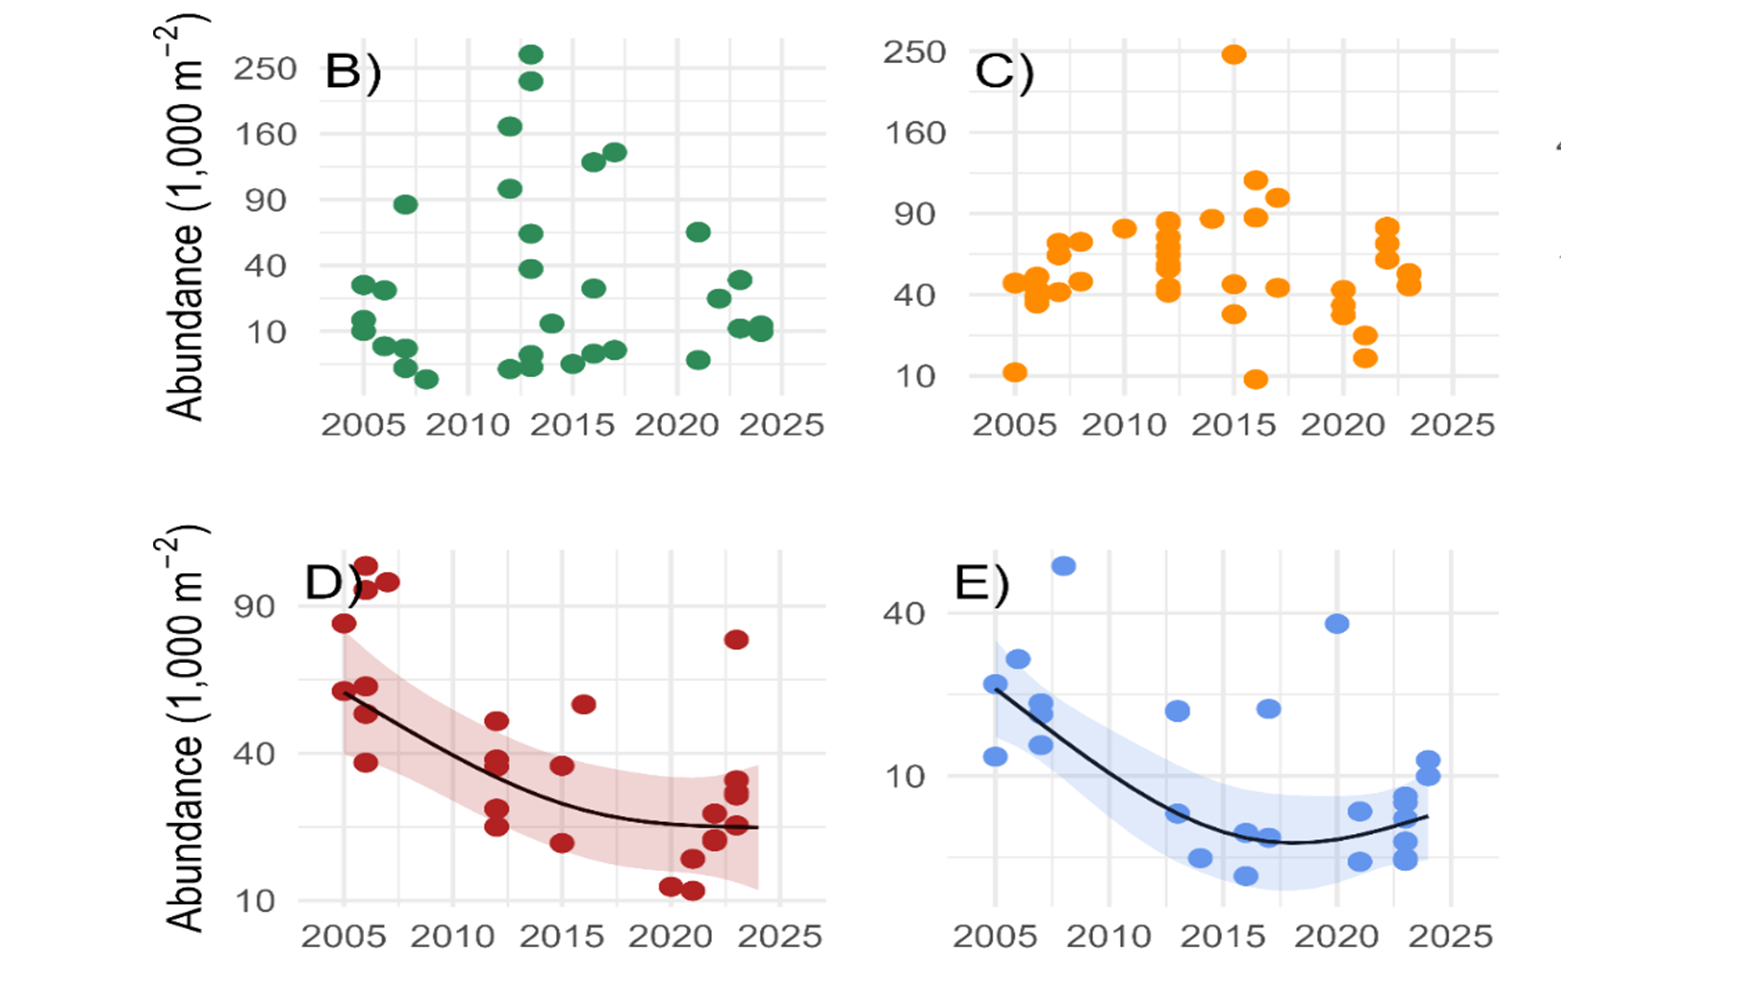
\includegraphics[width=24.42in]{SOE-NEFMC_files/figure-latex/zooplankton-season-1} 

}

\caption{Abundance (no $m^-2$) of *C. finmarchicus C3-C6 estimated from 200$\mu$ vertical ring net tows. Individual data with fitted lines.Data from 2005-2010: circles; 2011-2021:triangles; 2022-2024:squares) WBTS station seasonal abundance time series for B) spring, C) summer, D) fall, E)winter. Vertical lines denote season boudnaries. If the seasonal abundance time series is significant, GAM predictions are calculated with day of year set to 1, 100, 200, and 300 for winter, spring, summer, and fall, respectively.}\label{fig:zooplankton-season}
\end{figure}

\hypertarget{environmental-drivers}{%
\subparagraph{Environmental Drivers}\label{environmental-drivers}}

Fish production can also be directly related to the prevailing environmental conditions by altering metabolic (growth) and reproductive processes. Many species possess thermal tolerances and can experience stressful or lethal conditions if temperatures exceed certain levels. Extreme temperature at both the \href{https://noaa-edab.github.io/catalog/seasonal_oisst_anom.html}{surface} (Fig. \ref{fig:longterm-sst}) and \href{https://noaa-edab.github.io/catalog/bottom_temp_comp.html}{bottom} can exceed \href{https://noaa-edab.github.io/catalog/thermal_habitat_persistence.html}{thermal tolerance} limits for some fish. For example, 2012 had among the warmest surface and bottom temperatures (GB) in New England. A large proportion of the Georges Bank and Mid-Atlantic regions had bottom temperatures above the 15℃ thermal tolerance for most groundfish, with some days in the Mid-Atlantic exceeding the 24℃ potential mortality limit (Fig. ).
(Fig. \ref{fig:therm-hab-persist-2012}).

In 2024, only one \href{https://noaa-edab.github.io/catalog/heatwave_year.html}{surface marine heatwave} occurred throughout the entire U.S. Northeast Shelf due to the cooler ocean conditions observed in the region. This surface marine heatwave occurred in the Gulf of Maine starting on May 29th, peaking on June 7th, and lasting 12 days. This marine heatwave was not within the top 10 on record in terms of intesity.

\begin{figure}

{\centering \includegraphics{SOE-NEFMC_files/figure-latex/therm-hab-persist-2012-1} 

}

\caption{The number of days in 2024 where bottom temperature exceeds 15℃ (left) and 24℃ (right) based on the GLORYS 1/12 degree grid.}\label{fig:therm-hab-persist-2012}
\end{figure}

\href{https://noaa-edab.github.io/catalog/ocean_acidification.html}{Ocean acidification} (OA) risks vary among species and include reduced survival, growth, reproduction, and productivity, where high OA risk indicates potential negative effects to species. OA risk can also be heightened during colder conditions due to increased CO2 absorption by the water or by transport of high CO2 water masses (see \protect\hyperlink{highlights}{highlights section}). Higher OA risk conditions were observed for Atlantic sea scallop and longfin squid in Long Island Sound and the nearshore and mid shelf regions of the New Jersey shelf during summers of 2016, 2018, 2019, 2023, and 2024 (Fig. \ref{fig:oa-2024} ). The OA indicator observed on the Mid-Atlantic coastal shelf during summer 2024 was the most extreme recorded when compared to all of the years sampled (since 2007).

\begin{figure}

{\centering \includegraphics[width=1\linewidth]{SOE-NEFMC_files/figure-latex/oa-2024-1} 

}

\caption{Locations where bottom aragonite saturation state ($\Omega_{Arag}$; summer only: June-August) were at or below the laboratory-derived sensitivity level for Atlantic sea scallop (left panel) and longfin squid (right panel) for the time periods 2007-2022 (dark cyan) and 2023 only (magenta). Gray circles indicate locations where bottom $\Omega_{Arag}$ values were above the species specific sensitivity values.}\label{fig:oa-2024}
\end{figure}

Biological and oceanographic processes can affect the amount of oxygen present in the water column. During low oxygen (hypoxic) events, species' growth is negatively affected and very low oxygen can result in mortality. The duration and extent of hypoxic events is being monitored, but long-term shelf-wide observations are not yet available. However, \href{https://noaa-edab.github.io/catalog/observation_synthesis.html}{hypoxic events} were detected off the coast of New Jersey in 2023 and were potentially responsible for fish, lobster, and crab \href{https://sebsnjaesnews.rutgers.edu/2023/12/rutgers-scientists-observe-unusual-ocean-conditions-possibly-linked-to-mortality-in-marine-life-off-new-jersey/}{mortalities}. No hypoxic events were observed on the NE shelf in 2024.

\hypertarget{drivers-predation}{%
\subparagraph{Drivers: Predation}\label{drivers-predation}}

The abundance and distribution of predators can affect both the productivity and mortality rates on managed stocks. Predators can consume managed species or compete for the same resources resulting in increased natural mortality or declining productivity, respectively. The northeast shift in some \href{https://noaa-edab.github.io/catalog/HMS_species_distribution.html}{highly migratory species} (Fig. \ref{fig:protectedspp-dist-shifts}) indicates a change in the overlap between predators and prey. Since we also observe distribution shifts in both managed and forage species, the effect of changing predator distributions alone is difficult to quantify.

\href{https://noaa-edab.github.io/catalog/grayseal.html}{Gray seals} are fish predators with increasing populations in New England, however they are broad generalist feeders that do not generally target commercially-sized managed species. \href{https://noaa-edab.github.io/catalog/hms_stock_status.html}{Stock status} is mixed for Atlantic Highly Migratory Species (HMS) stocks (including sharks, swordfish, billfish, and tunas) occurring throughout the Northeast U.S. shelf. While there are several HMS species considered to be overfished or that have unknown stock status, the population status for some managed Atlantic sharks and tunas is at or above the biomass target, suggesting the potential for robust (or rebuilt) predator populations among these managed species. Stable predator populations suggest stable predation pressure on managed species, but increasing predator populations may reflect increasing predation pressure.

\hypertarget{future-considerations-2}{%
\paragraph{Future Considerations}\label{future-considerations-2}}

The processes that control fish productivity and mortality are dynamic, complex, and the result of the interactions between multiple system drivers. There is a real risk that short-term predictions in assessments and rebuilding plans that assume unchanging underlying conditions will not be as effective, given the observed ecological and environmental process changes documented throughout the report. Assumptions for species' growth, reproduction, and natural mortality should continue to be evaluated for individual species. With observations of system-wide productivity shifts of multiple managed stocks, more research is needed to determine whether regime shifts or ecosystem reorganization are occurring, and how this should be incorporated into management

\hypertarget{wind-risks}{%
\subsection{Other Ocean Uses: Offshore Wind}\label{wind-risks}}

\hypertarget{indicators-development-timeline-revenue-in-lease-areas-coastal-community-vulnerability}{%
\subsubsection{Indicators: development timeline, revenue in lease areas, coastal community vulnerability}\label{indicators-development-timeline-revenue-in-lease-areas-coastal-community-vulnerability}}

As of January 2025, 30 offshore \href{https://noaa-edab.github.io/catalog/wind_dev_speed.html}{wind development} projects are proposed for construction over the next decade in the Northeast (timelines and project data for 2024 are based on the \href{https://www.boem.gov/sites/default/files/documents/renewable-energy/state-activities/Ocean_Wind1_FEIS_App_F_Planned\%20Activities\%20Scenario.pdf}{Ocean Wind 1 Offshore Wind Farm Final Environmental Impact Statement. Volume II: Appendix F}). Offshore wind areas are anticipated to cover more than 2.3 million acres by 2030 in the Greater Atlantic region (Fig. \ref{fig:wind-proposed-dev}).

\begin{figure}

{\centering \includegraphics{SOE-NEFMC_files/figure-latex/wind-proposed-dev-1} 

}

\caption{Proposed wind development on the northeast shelf.}\label{fig:wind-proposed-dev}
\end{figure}

ust over 3,300 foundations and more than 12,000 miles of inter-array and offshore export cables are proposed to date. Since first reporting timeline indicators in 2021, construction years by 2030 have become increasingly uncertain with a wide range of estimated construction years being reported for some projects as reflected in the ``Estimated Construction Schedule'' column of Fig. \ref{fig:wind-dev-cumul2} below. The areas affected would be spread out such that it is unlikely that any one particular area would experience full development at one time. Construction of two projects in Southern New England (Vineyard Wind 1 and Revolution Wind) and two more projects in the Mid-Atlantic/New York Bight (Coastal Virginia Offshore Wind and Empire Wind 1) during 2024 has affected fisheries managed by the New England Fishery Management Council. It is likely that construction will begin on other projects in Southern New England and possibly the New York Bight during 2025 that will further affect regional fisheries.

Offshore floating wind is expected to be developed in the GOM. The Bureau of Ocean Energy Management (BOEM) leased four areas within the GOM for commercial development on October 29, 2024 (Fig. \ref{fig:wind-dev-cumul2}). BOEM also approved the state of Maine's application to lease 9,700 acres (15 square miles) for the first floating offshore wind research site in federal waters of the GOM, which could have up to 12 turbines.

NEFSC has partnered with the Responsible Ocean Development Alliance (RODA) and the University of Rhode Island to conduct an Integrated Ecosystem Assessment (IEA) of the interactions between offshore wind, fisheries, and the environment in the GOM. The IEA report will be similar to the State of the Ecosystem, but fully dedicated to impacts of offshore wind. Data from the IEA will be suitable for inclusion in the environmental impact statements for any projects in the GOM.

Based on federal vessel logbook data, \href{https://noaa-edab.github.io/catalog/wind_revenue.html}{commercial fishery revenue} rom trips in the current offshore wind lease areas represents 2-15\% of the total annual revenue for fisheries managed by the NEFMC from 2008-2023 (Table \ref{tab:wea-landings-rev}).Fishing revenue affected by offshore wind lease areas varies over time, but has largely declined over time. Maximum annual revenue for the fisheries with the most overlap with wind lease areas peaked at over \$52 million for the sea scallop fishery, \$2.5 million for monkfish, \$1.1 million for haddock, \$943,000 for pollock, \$840,000 for cod, just under \$700,000 for skates and redfish, \$662,000 for silver hake, and nearly \$600,000 for Atlantic herring (Fig. \ref{fig:wea-spp-rev}). The scallop fishery is mainly affected by lease areas in the Mid-Atlantic, as the Northern Area scallop fishery is outside of the GOM lease areas. However, substantial groundfish landings/revenues overlap with the GOM lease areas, as noted above. Individual groundfish species are more affected than others, with up to 15\% of historical annual revenues overlapping with existing lease areas for species such as yellowtail flounder (15\%), pollock (11\%) and 9\% for redfish and white hake (Table \ref{tab:wea-landings-rev}). Future fishery resource overlap with wind leases, especially scallops, may change due to species distribution shifts attributable to climate change and recruitment and larval dispersion pattern changes caused by hydrodynamic flow disruptions from turbine foundations, which could also affect fishery landings/revenue.

\begin{figure}

{\centering \includegraphics[width=0.9\linewidth]{SOE-NEFMC_files/figure-latex/wind-dev-cumul2-1} 

}

\caption{All Northeast Project areas by year construction ends (each project has 2 year construction period).}\label{fig:wind-dev-cumul2}
\end{figure}

\begin{figure}

{\centering \includegraphics{SOE-NEFMC_files/figure-latex/wea-spp-rev-1} 

}

\caption{Fishery revenues from NEFMC managed species in the Wind energy lease areas.}\label{fig:wea-spp-rev}
\end{figure}

\global\setlength{\Oldarrayrulewidth}{\arrayrulewidth}

\global\setlength{\Oldtabcolsep}{\tabcolsep}

\setlength{\tabcolsep}{0pt}

\renewcommand*{\arraystretch}{1}



\providecommand{\ascline}[3]{\noalign{\global\arrayrulewidth #1}\arrayrulecolor[HTML]{#2}\cline{#3}}

\begin{longtable}[c]{|p{2.00in}|p{2.00in}|p{2.00in}}

\caption{New\ England\ managed\ species\ Landings\ and\ Revenue\ from\ Wind\ Energy\ Areas.\ *Skates\ includes\ barndoor,\ winter,\ clearnose,\ smooth,\ little,\ and\ general\ skates\ reported\ in\ logbooks.}\label{tab:wea-landings-rev}\\

\ascline{1.5pt}{666666}{1-3}

\multicolumn{1}{>{\raggedright}m{\dimexpr 2in+0\tabcolsep}}{\textcolor[HTML]{000000}{\fontsize{9}{9}\selectfont{NEFMC,\ MAFMC,\ and\ ASMFC\ Managed\ Species}}} & \multicolumn{1}{>{\raggedleft}m{\dimexpr 2in+0\tabcolsep}}{\textcolor[HTML]{000000}{\fontsize{9}{9}\selectfont{Maximum\ Percent\ Total\ Annual\ Regional\ Species\ Landings}}} & \multicolumn{1}{>{\raggedleft}m{\dimexpr 2in+0\tabcolsep}}{\textcolor[HTML]{000000}{\fontsize{9}{9}\selectfont{Maximum\ Percent\ Total\ Annual\ Regional\ Species\ Revenue}}} \\

\ascline{1.5pt}{666666}{1-3}\endfirsthead \caption[]{New\ England\ managed\ species\ Landings\ and\ Revenue\ from\ Wind\ Energy\ Areas.\ *Skates\ includes\ barndoor,\ winter,\ clearnose,\ smooth,\ little,\ and\ general\ skates\ reported\ in\ logbooks.}\label{tab:wea-landings-rev}\\

\ascline{1.5pt}{666666}{1-3}

\multicolumn{1}{>{\raggedright}m{\dimexpr 2in+0\tabcolsep}}{\textcolor[HTML]{000000}{\fontsize{9}{9}\selectfont{NEFMC,\ MAFMC,\ and\ ASMFC\ Managed\ Species}}} & \multicolumn{1}{>{\raggedleft}m{\dimexpr 2in+0\tabcolsep}}{\textcolor[HTML]{000000}{\fontsize{9}{9}\selectfont{Maximum\ Percent\ Total\ Annual\ Regional\ Species\ Landings}}} & \multicolumn{1}{>{\raggedleft}m{\dimexpr 2in+0\tabcolsep}}{\textcolor[HTML]{000000}{\fontsize{9}{9}\selectfont{Maximum\ Percent\ Total\ Annual\ Regional\ Species\ Revenue}}} \\

\ascline{1.5pt}{666666}{1-3}\endhead



\multicolumn{1}{>{\raggedright}m{\dimexpr 2in+0\tabcolsep}}{\textcolor[HTML]{000000}{\fontsize{9}{9}\selectfont{Clearnose\ Skate*}}} & \multicolumn{1}{>{\raggedleft}m{\dimexpr 2in+0\tabcolsep}}{\textcolor[HTML]{000000}{\fontsize{9}{9}\selectfont{18}}} & \multicolumn{1}{>{\raggedleft}m{\dimexpr 2in+0\tabcolsep}}{\textcolor[HTML]{000000}{\fontsize{9}{9}\selectfont{20}}} \\





\multicolumn{1}{>{\raggedright}m{\dimexpr 2in+0\tabcolsep}}{\textcolor[HTML]{000000}{\fontsize{9}{9}\selectfont{Barndoor\ Skate*}}} & \multicolumn{1}{>{\raggedleft}m{\dimexpr 2in+0\tabcolsep}}{\textcolor[HTML]{000000}{\fontsize{9}{9}\selectfont{19}}} & \multicolumn{1}{>{\raggedleft}m{\dimexpr 2in+0\tabcolsep}}{\textcolor[HTML]{000000}{\fontsize{9}{9}\selectfont{18}}} \\





\multicolumn{1}{>{\raggedright}m{\dimexpr 2in+0\tabcolsep}}{\textcolor[HTML]{000000}{\fontsize{9}{9}\selectfont{Yellowtail\ Flounder}}} & \multicolumn{1}{>{\raggedleft}m{\dimexpr 2in+0\tabcolsep}}{\textcolor[HTML]{000000}{\fontsize{9}{9}\selectfont{15}}} & \multicolumn{1}{>{\raggedleft}m{\dimexpr 2in+0\tabcolsep}}{\textcolor[HTML]{000000}{\fontsize{9}{9}\selectfont{15}}} \\





\multicolumn{1}{>{\raggedright}m{\dimexpr 2in+0\tabcolsep}}{\textcolor[HTML]{000000}{\fontsize{9}{9}\selectfont{Little\ Skate}}} & \multicolumn{1}{>{\raggedleft}m{\dimexpr 2in+0\tabcolsep}}{\textcolor[HTML]{000000}{\fontsize{9}{9}\selectfont{12}}} & \multicolumn{1}{>{\raggedleft}m{\dimexpr 2in+0\tabcolsep}}{\textcolor[HTML]{000000}{\fontsize{9}{9}\selectfont{14}}} \\





\multicolumn{1}{>{\raggedright}m{\dimexpr 2in+0\tabcolsep}}{\textcolor[HTML]{000000}{\fontsize{9}{9}\selectfont{Pollock}}} & \multicolumn{1}{>{\raggedleft}m{\dimexpr 2in+0\tabcolsep}}{\textcolor[HTML]{000000}{\fontsize{9}{9}\selectfont{11}}} & \multicolumn{1}{>{\raggedleft}m{\dimexpr 2in+0\tabcolsep}}{\textcolor[HTML]{000000}{\fontsize{9}{9}\selectfont{11}}} \\





\multicolumn{1}{>{\raggedright}m{\dimexpr 2in+0\tabcolsep}}{\textcolor[HTML]{000000}{\fontsize{9}{9}\selectfont{Winter\ Skate}}} & \multicolumn{1}{>{\raggedleft}m{\dimexpr 2in+0\tabcolsep}}{\textcolor[HTML]{000000}{\fontsize{9}{9}\selectfont{10}}} & \multicolumn{1}{>{\raggedleft}m{\dimexpr 2in+0\tabcolsep}}{\textcolor[HTML]{000000}{\fontsize{9}{9}\selectfont{11}}} \\





\multicolumn{1}{>{\raggedright}m{\dimexpr 2in+0\tabcolsep}}{\textcolor[HTML]{000000}{\fontsize{9}{9}\selectfont{Redfish}}} & \multicolumn{1}{>{\raggedleft}m{\dimexpr 2in+0\tabcolsep}}{\textcolor[HTML]{000000}{\fontsize{9}{9}\selectfont{10}}} & \multicolumn{1}{>{\raggedleft}m{\dimexpr 2in+0\tabcolsep}}{\textcolor[HTML]{000000}{\fontsize{9}{9}\selectfont{9}}} \\





\multicolumn{1}{>{\raggedright}m{\dimexpr 2in+0\tabcolsep}}{\textcolor[HTML]{000000}{\fontsize{9}{9}\selectfont{White\ Hake}}} & \multicolumn{1}{>{\raggedleft}m{\dimexpr 2in+0\tabcolsep}}{\textcolor[HTML]{000000}{\fontsize{9}{9}\selectfont{9}}} & \multicolumn{1}{>{\raggedleft}m{\dimexpr 2in+0\tabcolsep}}{\textcolor[HTML]{000000}{\fontsize{9}{9}\selectfont{9}}} \\





\multicolumn{1}{>{\raggedright}m{\dimexpr 2in+0\tabcolsep}}{\textcolor[HTML]{000000}{\fontsize{9}{9}\selectfont{Atlantic\ Sea\ Scallop}}} & \multicolumn{1}{>{\raggedleft}m{\dimexpr 2in+0\tabcolsep}}{\textcolor[HTML]{000000}{\fontsize{9}{9}\selectfont{10}}} & \multicolumn{1}{>{\raggedleft}m{\dimexpr 2in+0\tabcolsep}}{\textcolor[HTML]{000000}{\fontsize{9}{9}\selectfont{9}}} \\





\multicolumn{1}{>{\raggedright}m{\dimexpr 2in+0\tabcolsep}}{\textcolor[HTML]{000000}{\fontsize{9}{9}\selectfont{Monkfish}}} & \multicolumn{1}{>{\raggedleft}m{\dimexpr 2in+0\tabcolsep}}{\textcolor[HTML]{000000}{\fontsize{9}{9}\selectfont{9}}} & \multicolumn{1}{>{\raggedleft}m{\dimexpr 2in+0\tabcolsep}}{\textcolor[HTML]{000000}{\fontsize{9}{9}\selectfont{8}}} \\





\multicolumn{1}{>{\raggedright}m{\dimexpr 2in+0\tabcolsep}}{\textcolor[HTML]{000000}{\fontsize{9}{9}\selectfont{Witch\ Flounder}}} & \multicolumn{1}{>{\raggedleft}m{\dimexpr 2in+0\tabcolsep}}{\textcolor[HTML]{000000}{\fontsize{9}{9}\selectfont{8}}} & \multicolumn{1}{>{\raggedleft}m{\dimexpr 2in+0\tabcolsep}}{\textcolor[HTML]{000000}{\fontsize{9}{9}\selectfont{7}}} \\





\multicolumn{1}{>{\raggedright}m{\dimexpr 2in+0\tabcolsep}}{\textcolor[HTML]{000000}{\fontsize{9}{9}\selectfont{Red\ Hake}}} & \multicolumn{1}{>{\raggedleft}m{\dimexpr 2in+0\tabcolsep}}{\textcolor[HTML]{000000}{\fontsize{9}{9}\selectfont{11}}} & \multicolumn{1}{>{\raggedleft}m{\dimexpr 2in+0\tabcolsep}}{\textcolor[HTML]{000000}{\fontsize{9}{9}\selectfont{7}}} \\





\multicolumn{1}{>{\raggedright}m{\dimexpr 2in+0\tabcolsep}}{\textcolor[HTML]{000000}{\fontsize{9}{9}\selectfont{Silver\ Hake}}} & \multicolumn{1}{>{\raggedleft}m{\dimexpr 2in+0\tabcolsep}}{\textcolor[HTML]{000000}{\fontsize{9}{9}\selectfont{8}}} & \multicolumn{1}{>{\raggedleft}m{\dimexpr 2in+0\tabcolsep}}{\textcolor[HTML]{000000}{\fontsize{9}{9}\selectfont{7}}} \\





\multicolumn{1}{>{\raggedright}m{\dimexpr 2in+0\tabcolsep}}{\textcolor[HTML]{000000}{\fontsize{9}{9}\selectfont{American\ Plaice}}} & \multicolumn{1}{>{\raggedleft}m{\dimexpr 2in+0\tabcolsep}}{\textcolor[HTML]{000000}{\fontsize{9}{9}\selectfont{6}}} & \multicolumn{1}{>{\raggedleft}m{\dimexpr 2in+0\tabcolsep}}{\textcolor[HTML]{000000}{\fontsize{9}{9}\selectfont{7}}} \\





\multicolumn{1}{>{\raggedright}m{\dimexpr 2in+0\tabcolsep}}{\textcolor[HTML]{000000}{\fontsize{9}{9}\selectfont{Haddock}}} & \multicolumn{1}{>{\raggedleft}m{\dimexpr 2in+0\tabcolsep}}{\textcolor[HTML]{000000}{\fontsize{9}{9}\selectfont{6}}} & \multicolumn{1}{>{\raggedleft}m{\dimexpr 2in+0\tabcolsep}}{\textcolor[HTML]{000000}{\fontsize{9}{9}\selectfont{6}}} \\





\multicolumn{1}{>{\raggedright}m{\dimexpr 2in+0\tabcolsep}}{\textcolor[HTML]{000000}{\fontsize{9}{9}\selectfont{Smooth\ Skate*}}} & \multicolumn{1}{>{\raggedleft}m{\dimexpr 2in+0\tabcolsep}}{\textcolor[HTML]{000000}{\fontsize{9}{9}\selectfont{10}}} & \multicolumn{1}{>{\raggedleft}m{\dimexpr 2in+0\tabcolsep}}{\textcolor[HTML]{000000}{\fontsize{9}{9}\selectfont{6}}} \\





\multicolumn{1}{>{\raggedright}m{\dimexpr 2in+0\tabcolsep}}{\textcolor[HTML]{000000}{\fontsize{9}{9}\selectfont{Atlantic\ Cod}}} & \multicolumn{1}{>{\raggedleft}m{\dimexpr 2in+0\tabcolsep}}{\textcolor[HTML]{000000}{\fontsize{9}{9}\selectfont{5}}} & \multicolumn{1}{>{\raggedleft}m{\dimexpr 2in+0\tabcolsep}}{\textcolor[HTML]{000000}{\fontsize{9}{9}\selectfont{5}}} \\





\multicolumn{1}{>{\raggedright}m{\dimexpr 2in+0\tabcolsep}}{\textcolor[HTML]{000000}{\fontsize{9}{9}\selectfont{Atlantic\ Halibut*}}} & \multicolumn{1}{>{\raggedleft}m{\dimexpr 2in+0\tabcolsep}}{\textcolor[HTML]{000000}{\fontsize{9}{9}\selectfont{5}}} & \multicolumn{1}{>{\raggedleft}m{\dimexpr 2in+0\tabcolsep}}{\textcolor[HTML]{000000}{\fontsize{9}{9}\selectfont{5}}} \\





\multicolumn{1}{>{\raggedright}m{\dimexpr 2in+0\tabcolsep}}{\textcolor[HTML]{000000}{\fontsize{9}{9}\selectfont{Winter\ Flounder}}} & \multicolumn{1}{>{\raggedleft}m{\dimexpr 2in+0\tabcolsep}}{\textcolor[HTML]{000000}{\fontsize{9}{9}\selectfont{4}}} & \multicolumn{1}{>{\raggedleft}m{\dimexpr 2in+0\tabcolsep}}{\textcolor[HTML]{000000}{\fontsize{9}{9}\selectfont{4}}} \\





\multicolumn{1}{>{\raggedright}m{\dimexpr 2in+0\tabcolsep}}{\textcolor[HTML]{000000}{\fontsize{9}{9}\selectfont{Offshore\ Hake}}} & \multicolumn{1}{>{\raggedleft}m{\dimexpr 2in+0\tabcolsep}}{\textcolor[HTML]{000000}{\fontsize{9}{9}\selectfont{17}}} & \multicolumn{1}{>{\raggedleft}m{\dimexpr 2in+0\tabcolsep}}{\textcolor[HTML]{000000}{\fontsize{9}{9}\selectfont{3}}} \\





\multicolumn{1}{>{\raggedright}m{\dimexpr 2in+0\tabcolsep}}{\textcolor[HTML]{000000}{\fontsize{9}{9}\selectfont{Spiny\ Dogfish}}} & \multicolumn{1}{>{\raggedleft}m{\dimexpr 2in+0\tabcolsep}}{\textcolor[HTML]{000000}{\fontsize{9}{9}\selectfont{2}}} & \multicolumn{1}{>{\raggedleft}m{\dimexpr 2in+0\tabcolsep}}{\textcolor[HTML]{000000}{\fontsize{9}{9}\selectfont{3}}} \\





\multicolumn{1}{>{\raggedright}m{\dimexpr 2in+0\tabcolsep}}{\textcolor[HTML]{000000}{\fontsize{9}{9}\selectfont{Windowpane\ Flounder*}}} & \multicolumn{1}{>{\raggedleft}m{\dimexpr 2in+0\tabcolsep}}{\textcolor[HTML]{000000}{\fontsize{9}{9}\selectfont{3}}} & \multicolumn{1}{>{\raggedleft}m{\dimexpr 2in+0\tabcolsep}}{\textcolor[HTML]{000000}{\fontsize{9}{9}\selectfont{3}}} \\





\multicolumn{1}{>{\raggedright}m{\dimexpr 2in+0\tabcolsep}}{\textcolor[HTML]{000000}{\fontsize{9}{9}\selectfont{Atlantic\ Herring}}} & \multicolumn{1}{>{\raggedleft}m{\dimexpr 2in+0\tabcolsep}}{\textcolor[HTML]{000000}{\fontsize{9}{9}\selectfont{3}}} & \multicolumn{1}{>{\raggedleft}m{\dimexpr 2in+0\tabcolsep}}{\textcolor[HTML]{000000}{\fontsize{9}{9}\selectfont{2}}} \\





\multicolumn{1}{>{\raggedright}m{\dimexpr 2in+0\tabcolsep}}{\textcolor[HTML]{000000}{\fontsize{9}{9}\selectfont{Thorny\ Skate*}}} & \multicolumn{1}{>{\raggedleft}m{\dimexpr 2in+0\tabcolsep}}{\textcolor[HTML]{000000}{\fontsize{9}{9}\selectfont{2}}} & \multicolumn{1}{>{\raggedleft}m{\dimexpr 2in+0\tabcolsep}}{\textcolor[HTML]{000000}{\fontsize{9}{9}\selectfont{2}}} \\





\multicolumn{1}{>{\raggedright}m{\dimexpr 2in+0\tabcolsep}}{\textcolor[HTML]{000000}{\fontsize{9}{9}\selectfont{Red\ Crab}}} & \multicolumn{1}{>{\raggedleft}m{\dimexpr 2in+0\tabcolsep}}{\textcolor[HTML]{000000}{\fontsize{9}{9}\selectfont{2}}} & \multicolumn{1}{>{\raggedleft}m{\dimexpr 2in+0\tabcolsep}}{\textcolor[HTML]{000000}{\fontsize{9}{9}\selectfont{2}}} \\





\multicolumn{1}{>{\raggedright}m{\dimexpr 2in+0\tabcolsep}}{\textcolor[HTML]{000000}{\fontsize{9}{9}\selectfont{American\ Lobster}}} & \multicolumn{1}{>{\raggedleft}m{\dimexpr 2in+0\tabcolsep}}{\textcolor[HTML]{000000}{\fontsize{9}{9}\selectfont{1}}} & \multicolumn{1}{>{\raggedleft}m{\dimexpr 2in+0\tabcolsep}}{\textcolor[HTML]{000000}{\fontsize{9}{9}\selectfont{2}}} \\





\multicolumn{1}{>{\raggedright}m{\dimexpr 2in+0\tabcolsep}}{\textcolor[HTML]{000000}{\fontsize{9}{9}\selectfont{Atlantic\ Wolffish*}}} & \multicolumn{1}{>{\raggedleft}m{\dimexpr 2in+0\tabcolsep}}{\textcolor[HTML]{000000}{\fontsize{9}{9}\selectfont{2}}} & \multicolumn{1}{>{\raggedleft}m{\dimexpr 2in+0\tabcolsep}}{\textcolor[HTML]{000000}{\fontsize{9}{9}\selectfont{1}}} \\

\ascline{1.5pt}{666666}{1-3}



\end{longtable}



\arrayrulecolor[HTML]{000000}

\global\setlength{\arrayrulewidth}{\Oldarrayrulewidth}

\global\setlength{\tabcolsep}{\Oldtabcolsep}

\renewcommand*{\arraystretch}{1}

Social vulnerabilities of communities are priority concerns with offshore wind development and fisheries impacts in the Northeast, and the impacts of offshore wind development are expected to differentially \href{https://noaa-edab.github.io/catalog/wind_port.html}{impact specific coastal communities}. Additionally, impacts of offshore wind development may unevenly affect individual operators, with some permit holders deriving a much higher proportion of revenue from wind areas than the port-based mean.

\begin{figure}

\includegraphics{SOE-NEFMC_files/figure-latex/wea-port-rev-1} \hfill{}

\caption{Percent of port fisheries revenue from Wind Energy Areas (WEA) in descending order from most to least port fisheries revenue from WEA.}\label{fig:wea-port-rev}
\end{figure}

For example, Little Compton, RI had a minimum of 17\% and maximum of 32\% overlap of wind energy revenue to the total port revenue between 2008-2023 (Fig. \ref{fig:wea-port-rev}). BOEM reports that cumulative offshore wind development (if all proposed projects are developed) could have moderate impacts on low-income members of vulnerable communities who work in the commercial fishing and for-hire fishing industry due to disruptions to fish populations, restrictions on navigation, and increased vessel traffic as well as existing vulnerabilities of low-income workers to economic impacts.

Top fishing communities with high \href{https://noaa-edab.github.io/catalog/engagement.html}{socio-demographic concerns} such as New Bedford, MA and New London, CT should be considered in decision making to reduce the social and economic impacts and aid in the resilience and adaptive capacity of underserved communities. These two ports are also undergoing significant changes to support offshore wind development port infrastructure needs. Socio-demographic concerns also highlight communities where further resources are needed to reach underserved and underrepresented groups and create opportunities for, and directly involve, these groups in the decision-making process.

\begin{figure}

\includegraphics{SOE-NEFMC_files/figure-latex/wind-rev-MAB-NEFMC-1} \hfill{}

\caption{Percent of Mid-Atlantic port revenue with majority NEFMC landings from Wind Energy Areas (WEA) in descending order from most to least port fisheries revenue from WEA.}\label{fig:wind-rev-MAB-NEFMC}
\end{figure}

\hypertarget{implications-6}{%
\subsubsection{Implications}\label{implications-6}}

Current plans for rapid buildout of offshore wind in a patchwork of areas spreads the impacts differentially throughout the region (Fig. \ref{fig:wind-dev-cumul2}).

Up to 12\% of total average revenue for major New England commercial species in lease areas could be forgone, or reduced, and associated effort displaced if all sites are developed. Displaced fishing effort can alter historic fishing areas, timing, and methods, which can in turn change habitat, species (managed and protected), and fleet interactions. Several factors, including fishery regulations, fishery availability, and user conflicts affect where, when, and how fishing effort may be displaced, along with impacts to and responses of affected fish species.

Planned development \href{https://noaa-edab.github.io/catalog/persistent_hotspots.html}{overlaps NARW} mother and calf migration corridors and a significant foraging habitat that is used throughout the year in addition to one of the only known winter foraging areas (Fig. \ref{fig:whales-wind}). Turbine presence and extraction of energy from the system could alter local oceanography and may affect right whale prey availability. For example, persistent foraging hotspots of right whales and seabirds overlap on Nantucket Shoals, where unique hydrography aggregates enhanced prey densities. Wind leases (OCS-A 0521 and OCS-A 0522) currently intersect these hotspots on the southwestern corner of Nantucket Shoals and a prominent tidal front associated with invertebrate prey swarms important to seabirds and possibly right whales. Proposed wind development areas also bring increased vessel strike risk from construction and operation vessels. In addition, there are a number of potential impacts to whales from pile driving and operational noise such as displacement, increased levels of communication masking, and elevated stress hormones.

Proposed wind development areas interact with the region's federal scientific surveys. Scientific surveys are impacted by offshore wind in four ways:

\begin{enumerate}
\def\labelenumi{\arabic{enumi}.}
\tightlist
\item
  Exclusion of NOAA Fisheries' sampling platforms from the wind development area due to operational and safety limitations
\item
  Impacts on the random-stratified statistical design that is the basis for scientific assessments, advice, and analyses;
\item
  Alteration of benthic and pelagic habitats, and airspace in and around the wind energy development, requiring new designs and methods to sample new habitats
\item
  Reduced sampling productivity through navigation impacts of wind energy infrastructure on aerial and vessel survey operations
\end{enumerate}

Increased vessel transit between stations may decrease data collections that are already limited by annual days-at-sea day allocations. As of 2024, the total survey area overlap ranges from 1-70\% for all Greater Atlantic federal surveys. Individual survey strata have significant interaction with wind energy development, including the sea scallop survey (up to 96\% of individual strata) and the bottom trawl survey (BTS, up to 60\% strata overlap). Additionally, up to 50\% of the southern New England North Atlantic right whale survey's area overlaps with proposed project areas and a region-wide survey mitigation program is underway.

The increase of offshore wind development can have both positive (e.g., employment opportunities) and negative (e.g., space-use conflicts) sociocultural effects. Continued increase in coastal development and gentrification pressure has resulted in loss of fishing infrastructure space within ports. Understanding these existing pressures can help avoid and mitigate negative impacts to our shore support industry and communities dependent on fishing. Some of the communities with the highest fisheries revenue overlap with offshore wind development areas that are also vulnerable to gentrification pressure are Point Judith and Newport, RI; and Boston and New Bedford, MA.

\begin{figure}

{\centering \includegraphics[width=0.6\linewidth]{SOE-NEFMC_files/figure-latex/whales-wind-1} 

}

\caption{Northern Right Whale persistent hotspots and Wind Energy Areas. Areas outlined in black show active or proposed wind energy leases.}\label{fig:whales-wind}
\end{figure}
\newpage

\hypertarget{highlights}{%
\subsubsection{2024 Highlights}\label{highlights}}

This section intends to provide a record of noteworthy observations reported in 2024 across the Northeast U.S. region. The full ecosystem and fisheries impacts of many of these observations are still to be determined. They should, however, be noted and considered in future analyses and management decisions.

2024 global sea surface and air temperatures exceeded 2023 as the warmest year on record, but colder than average temperatures were observed in the Northeast U.S. Oceanographic and ecological conditions in the Northwest Atlantic were markedly different in 2024 compared to recent years.

\hypertarget{northwest-atlantic-phenomena}{%
\paragraph{Northwest Atlantic Phenomena}\label{northwest-atlantic-phenomena}}

Late 2023 and early 2024 observations indicate movement of cooler and fresher water into the Northwest Atlantic. Anomalously cold and low salinity conditions were recorded throughout the Northeast Shelf and were widespread across the Slope Sea. These cooler and fresher conditions are linked to the southward movement of the eastern portion of the \href{https://noaa-edab.github.io/catalog/gsi.html}{Gulf Stream} and an increased influx of Labrador Slope and Scotian Shelf water into the system.

\begin{figure}

{\centering \includegraphics[width=22.92in]{SOE-NEFMC_files/figure-latex/slopesea-1} 

}

\caption{February 2024 sea surface temperature difference compared to the February 2000-2020 long-term mean from the NOAA Advanced Clear-Sky Processor for Ocean (ACSPO) Super-collated SST.}\label{fig:slopesea}
\end{figure}

Labrador Slope water accounted for more than 50\% of the \href{https://noaa-edab.github.io/catalog/slopewater.html}{source water} entering the Gulf of Maine through the Northeast Channel (Fig. \ref{fig.slopewater}). The increased influx of Labrador Slope and Scotian Shelf water resulted in colder and fresher conditions throughout the Northwest Atlantic and contributed to the Mid-Atlantic \href{https://noaa-edab.github.io/catalog/cold_pool.html}{cold pool}. The cold pool area was larger and colder than recent years and more similar to the historical mean (1993-2020).

\begin{figure}

{\centering \includegraphics{SOE-NEFMC_files/figure-latex/slopewater-1} 

}

\caption{The proportion of Warm Slope Water (WSW) and Labrador Slope Water (LSW) enter the Gulf of Maine through the Northeast Channel. The orange and teal dashed lines represent the long-term proportion averages for the WSW and LSW respectively.}\label{fig:slopewater}
\end{figure}

\hypertarget{northeast-shelf-and-local-phenomena}{%
\paragraph{Northeast Shelf and Local Phenomena}\label{northeast-shelf-and-local-phenomena}}

The influx of the northern waters is likely linked to multiple observations across the Northeast Shelf including the uncommon presence of Arctic Calanus zooplankton species in the Gulf of Maine, delayed migration of many species, and redistribution of some species. Several members of the fishing community noted delayed migration of species into typical fishing grounds. In particular, they attributed the delayed migration of longfin squid, black sea bass, and haddock to the cooler water temperatures. Many also reported redistribution of some species. Specifically, pollock, bluefin tuna, Atlantic mackerel, longfin squid, bluefish, and bonito were observed in surprising or unusual locations. Some species, such as Atlantic mackerel, were reported outside of typical fishing grounds and in higher abundance compared to recent years. Anglers also reported good catches of red drum in Chesapeake Bay and record high (since 1995) numbers were observed at Poplar Island survey location.

In the summer, Chesapeake Bay recorded warm temperatures and low bottom water dissolved oxygen that resulted in less than suitable habitat for species such as striped bass and blue crabs. These poor conditions can affect their distribution, growth, and survival. Additionally, lower than average spring and summer salinity negatively impacted oyster hatchery operations and increased the area of available habitat for invasive blue catfish, potentially increasing predation on blue crabs and other important finfish species.

During the summer months there were multiple prolonged upwelling events that brought cold water to the surface off the New Jersey coast. There was also an atypical phytoplankton bloom south of Long Island in late June to early July 2024, possibly linked to an upwelling event (Fig. \ref{fig:cocbloom}). The bloom was dominated by coccolithophores, which have an exoskeleton made up of calcium carbonate plates that can turn the water an opaque turquoise color. Large blooms of coccolithophores are unusual in this region, but they are not considered harmful and are grazed by zooplankton. Additionally, there were observations of multiple whale species aggregating near the Hudson Canyon between May and August.

\begin{figure}

{\centering \includegraphics[width=0.65\linewidth]{SOE-NEFMC_files/figure-latex/cocobloom-1} 

}

\caption{An OLCI Sentinel 3A true color image with enhanced contrast captured on July 2, 2024. Coccolithophores shed their coccolith plates during the later stages of the bloom cycle, which results in the milky turquoise water color (Image credit: NOAA STAR, OCView and Ocean Color Science Team).}\label{fig:cocobloom}
\end{figure}

Summer bottom \href{https://noaa-edab.github.io/catalog/ocean_acidification.html}{ocean acidification (OA)} risk in the Mid-Atlantic was the highest recorded since sampling began in 2007. High OA risk is measured as low aragonite saturation state(\(\Omega\)). Similarly, the winter/early spring \href{https://noaa-edab.github.io/catalog/gom_acidification.html}{Gulf of Maine surface OA risk} was significantly above the climatological average and near the sensitivity levels for cod (\(\Omega\)\textless1.19) and lobster (\(\Omega\)\textless1.09) (Fig.\ref{fig:GOMoa}). These observations were likely driven by the greater volume of fresher, less-buffered Labrador Slope water entering the Gulf of Maine and Mid-Atlantic. The 2023 and 2024 high summer OA risk has increased the extent of potentially unfavorable habitat for Atlantic sea scallops (\(\Omega\)\textless1.1) and longfin squid (\(\Omega\)\textless0.96). Additionally, for the first time, high OA risk conditions were observed outside of summer (fall for both species and spring for Atlantic sea scallops).

\begin{figure}

{\centering \includegraphics[width=22.92in]{SOE-NEFMC_files/figure-latex/GOMoa-1} 

}

\caption{GOM OA}\label{fig:GOMoa}
\end{figure}

In contrast to the documented die-off of scallops in the Mid-Atlantic Elephant Trunk region between the 2022 and 2023 surveys, in 2024 there was strong scallop recruitment in the southeastern portion of the Nantucket Lightship Area.

\hypertarget{contributors}{%
\section{Contributors}\label{contributors}}

\textbf{Editors} (NOAA NMFS Northeast Fisheries Science Center, NEFSC): Joseph Caracappa, Sarah Gaichas, Andrew Beet, Brandon Beltz, Geret DePiper, Kimberly Hyde, Scott Large, Sean Lucey, Laurel Smith.

\newpage

\hypertarget{document-orientation}{%
\section{Document Orientation}\label{document-orientation}}

The figure format is illustrated in Fig \ref{fig:docformat}a. Trend lines are shown when the slope is significantly different from 0 at the p \textless{} 0.05 level. An orange line signifies an overall positive trend, and purple signifies a negative trend. To minimize bias introduced by small sample size, no trend is fit for \textless{} 30 year time series. Dashed lines represent mean values of time series unless the indicator is an anomaly, in which case the dashed line is equal to 0. Shaded regions indicate the past ten years. If there are no new data for 2020, the shaded region will still cover this time period. The spatial scale of indicators is either coastwide, New England states (Connecticut, Rhode Island, Massachusetts, New Hampshire, and Maine), or at one of the two Ecosystem Production Units (EPUs, Fig. \ref{fig:docformat}b) levels in the region, Georges Bank (GB) or Gulf of Maine (GOM).

\begin{figure}

{\centering \includegraphics{SOE-NEFMC_files/figure-latex/docformat-1} 

}

\caption{Document orientation. a. Key to figures. b.The Northeast Large Marine Ecosystem.}\label{fig:docformat}
\end{figure}

Fish and invertebrates are aggregated into similar \href{https://noaa-edab.github.io/catalog/species_groupings.html}{feeding guild categories} (Table \ref{tab:species-groupings}) to evaluate ecosystem level trends in predators and prey.

\global\setlength{\Oldarrayrulewidth}{\arrayrulewidth}

\global\setlength{\Oldtabcolsep}{\tabcolsep}

\setlength{\tabcolsep}{0pt}

\renewcommand*{\arraystretch}{1.5}



\providecommand{\ascline}[3]{\noalign{\global\arrayrulewidth #1}\arrayrulecolor[HTML]{#2}\cline{#3}}

\begin{longtable}[c]{|p{1.00in}|p{1.00in}|p{1.00in}|p{1.00in}|p{3.00in}}

\caption{Feeding\ guilds\ and\ management\ bodies.}\label{tab:species-groupings}\\

\ascline{1.5pt}{666666}{1-5}

\multicolumn{1}{>{\raggedright}m{\dimexpr 1in+0\tabcolsep}}{\textcolor[HTML]{000000}{\fontsize{8}{8}\selectfont{Guild}}} & \multicolumn{1}{>{\raggedright}m{\dimexpr 1in+0\tabcolsep}}{\textcolor[HTML]{000000}{\fontsize{8}{8}\selectfont{MAFMC}}} & \multicolumn{1}{>{\raggedright}m{\dimexpr 1in+0\tabcolsep}}{\textcolor[HTML]{000000}{\fontsize{8}{8}\selectfont{Joint}}} & \multicolumn{1}{>{\raggedright}m{\dimexpr 1in+0\tabcolsep}}{\textcolor[HTML]{000000}{\fontsize{8}{8}\selectfont{NEFMC}}} & \multicolumn{1}{>{\raggedright}m{\dimexpr 3in+0\tabcolsep}}{\textcolor[HTML]{000000}{\fontsize{8}{8}\selectfont{State\ or\ Other}}} \\

\ascline{1.5pt}{666666}{1-5}\endfirsthead \caption[]{Feeding\ guilds\ and\ management\ bodies.}\label{tab:species-groupings}\\

\ascline{1.5pt}{666666}{1-5}

\multicolumn{1}{>{\raggedright}m{\dimexpr 1in+0\tabcolsep}}{\textcolor[HTML]{000000}{\fontsize{8}{8}\selectfont{Guild}}} & \multicolumn{1}{>{\raggedright}m{\dimexpr 1in+0\tabcolsep}}{\textcolor[HTML]{000000}{\fontsize{8}{8}\selectfont{MAFMC}}} & \multicolumn{1}{>{\raggedright}m{\dimexpr 1in+0\tabcolsep}}{\textcolor[HTML]{000000}{\fontsize{8}{8}\selectfont{Joint}}} & \multicolumn{1}{>{\raggedright}m{\dimexpr 1in+0\tabcolsep}}{\textcolor[HTML]{000000}{\fontsize{8}{8}\selectfont{NEFMC}}} & \multicolumn{1}{>{\raggedright}m{\dimexpr 3in+0\tabcolsep}}{\textcolor[HTML]{000000}{\fontsize{8}{8}\selectfont{State\ or\ Other}}} \\

\ascline{1.5pt}{666666}{1-5}\endhead



\multicolumn{1}{>{\raggedright}m{\dimexpr 1in+0\tabcolsep}}{\textcolor[HTML]{000000}{\fontsize{8}{8}\selectfont{Apex\ Predator}}} & \multicolumn{1}{>{\raggedright}m{\dimexpr 1in+0\tabcolsep}}{\textcolor[HTML]{000000}{\fontsize{8}{8}\selectfont{}}} & \multicolumn{1}{>{\raggedright}m{\dimexpr 1in+0\tabcolsep}}{\textcolor[HTML]{000000}{\fontsize{8}{8}\selectfont{}}} & \multicolumn{1}{>{\raggedright}m{\dimexpr 1in+0\tabcolsep}}{\textcolor[HTML]{000000}{\fontsize{8}{8}\selectfont{}}} & \multicolumn{1}{>{\raggedright}m{\dimexpr 3in+0\tabcolsep}}{\textcolor[HTML]{000000}{\fontsize{8}{8}\selectfont{shark\ uncl,\ swordfish,\ yellowfin\ tuna,\ bluefin\ tuna}}} \\





\multicolumn{1}{>{\raggedright}m{\dimexpr 1in+0\tabcolsep}}{\textcolor[HTML]{000000}{\fontsize{8}{8}\selectfont{Piscivore}}} & \multicolumn{1}{>{\raggedright}m{\dimexpr 1in+0\tabcolsep}}{\textcolor[HTML]{000000}{\fontsize{8}{8}\selectfont{summer\ flounder,\ bluefish,\ northern\ shortfin\ squid,\ longfin\ squid}}} & \multicolumn{1}{>{\raggedright}m{\dimexpr 1in+0\tabcolsep}}{\textcolor[HTML]{000000}{\fontsize{8}{8}\selectfont{spiny\ dogfish,\ goosefish}}} & \multicolumn{1}{>{\raggedright}m{\dimexpr 1in+0\tabcolsep}}{\textcolor[HTML]{000000}{\fontsize{8}{8}\selectfont{winter\ skate,\ clearnose\ skate,\ thorny\ skate,\ offshore\ hake,\ silver\ hake,\ atlantic\ cod,\ pollock,\ white\ hake,\ red\ hake,\ atlantic\ halibut,\ acadian\ redfish}}} & \multicolumn{1}{>{\raggedright}m{\dimexpr 3in+0\tabcolsep}}{\textcolor[HTML]{000000}{\fontsize{8}{8}\selectfont{sea\ lamprey,\ sandbar\ shark,\ atlantic\ angel\ shark,\ atlantic\ torpedo,\ conger\ eel,\ spotted\ hake,\ cusk,\ fourspot\ flounder,\ windowpane,\ john\ dory,\ atlantic\ cutlassfish,\ blue\ runner,\ striped\ bass,\ weakfish,\ sea\ raven,\ northern\ stargazer,\ banded\ rudderfish,\ atlantic\ sharpnose\ shark,\ inshore\ lizardfish,\ atlantic\ brief\ squid,\ northern\ sennet,\ king\ mackerel,\ spanish\ mackerel}}} \\





\multicolumn{1}{>{\raggedright}m{\dimexpr 1in+0\tabcolsep}}{\textcolor[HTML]{000000}{\fontsize{8}{8}\selectfont{Planktivore}}} & \multicolumn{1}{>{\raggedright}m{\dimexpr 1in+0\tabcolsep}}{\textcolor[HTML]{000000}{\fontsize{8}{8}\selectfont{atlantic\ mackerel,\ chub\ mackerel,\ butterfish}}} & \multicolumn{1}{>{\raggedright}m{\dimexpr 1in+0\tabcolsep}}{\textcolor[HTML]{000000}{\fontsize{8}{8}\selectfont{}}} & \multicolumn{1}{>{\raggedright}m{\dimexpr 1in+0\tabcolsep}}{\textcolor[HTML]{000000}{\fontsize{8}{8}\selectfont{atlantic\ herring}}} & \multicolumn{1}{>{\raggedright}m{\dimexpr 3in+0\tabcolsep}}{\textcolor[HTML]{000000}{\fontsize{8}{8}\selectfont{harvestfishes,\ smelts,\ round\ herring,\ alewife,\ blueback\ herring,\ american\ shad,\ menhaden,\ bay\ anchovy,\ striped\ anchovy,\ rainbow\ smelt,\ atlantic\ argentine,\ slender\ snipe\ eel,\ atlantic\ silverside,\ northern\ pipefish,\ atlantic\ moonfish,\ lookdown,\ blackbelly\ rosefish,\ lumpfish,\ northern\ sand\ lance,\ atlantic\ saury,\ mackerel\ scad,\ bigeye\ scad,\ round\ scad,\ rough\ scad,\ silver\ rag,\ weitzmans\ pearlsides,\ atlantic\ soft\ pout,\ sevenspine\ bay\ shrimp,\ pink\ glass\ shrimp,\ polar\ lebbeid,\ friendly\ blade\ shrimp,\ bristled\ longbeak,\ aesop\ shrimp,\ norwegian\ shrimp,\ northern\ shrimp,\ brown\ rock\ shrimp,\ atlantic\ thread\ herring,\ spanish\ sardine,\ atlantic\ bumper,\ harvestfish,\ striated\ argentine,\ silver\ anchovy}}} \\





\multicolumn{1}{>{\raggedright}m{\dimexpr 1in+0\tabcolsep}}{\textcolor[HTML]{000000}{\fontsize{8}{8}\selectfont{Benthivore}}} & \multicolumn{1}{>{\raggedright}m{\dimexpr 1in+0\tabcolsep}}{\textcolor[HTML]{000000}{\fontsize{8}{8}\selectfont{black\ sea\ bass,\ scup,\ tilefish}}} & \multicolumn{1}{>{\raggedright}m{\dimexpr 1in+0\tabcolsep}}{\textcolor[HTML]{000000}{\fontsize{8}{8}\selectfont{}}} & \multicolumn{1}{>{\raggedright}m{\dimexpr 1in+0\tabcolsep}}{\textcolor[HTML]{000000}{\fontsize{8}{8}\selectfont{barndoor\ skate,\ rosette\ skate,\ little\ skate,\ smooth\ skate,\ haddock,\ american\ plaice,\ yellowtail\ flounder,\ winter\ flounder,\ witch\ flounder,\ atlantic\ wolffish,\ ocean\ pout,\ crab,red\ deepsea}}} & \multicolumn{1}{>{\raggedright}m{\dimexpr 3in+0\tabcolsep}}{\textcolor[HTML]{000000}{\fontsize{8}{8}\selectfont{crab,unc,\ hagfish,\ porgy,red,\ sea\ bass,nk,\ atlantic\ hagfish,\ roughtail\ stingray,\ smooth\ dogfish,\ chain\ dogfish,\ bluntnose\ stingray,\ bullnose\ ray,\ southern\ stingray,\ longfin\ hake,\ fourbeard\ rockling,\ marlin-spike,\ gulf\ stream\ flounder,\ longspine\ snipefish,\ blackmouth\ bass,\ threespine\ stickleback,\ smallmouth\ flounder,\ hogchoker,\ bigeye,\ atlantic\ croaker,\ pigfish,\ northern\ kingfish,\ silver\ perch,\ spot,\ deepbody\ boarfish,\ sculpin\ uncl,\ moustache\ sculpin,\ longhorn\ sculpin,\ alligatorfish,\ grubby,\ atlantic\ seasnail,\ northern\ searobin,\ striped\ searobin,\ armored\ searobin,\ cunner,\ tautog,\ snakeblenny,\ daubed\ shanny,\ radiated\ shanny,\ red\ goatfish,\ striped\ cusk-eel,\ wolf\ eelpout,\ wrymouth,\ fawn\ cusk-eel,\ northern\ puffer,\ striped\ burrfish,\ planehead\ filefish,\ gray\ triggerfish,\ shortnose\ greeneye,\ beardfish,\ cownose\ ray,\ american\ lobster,\ cancer\ crab\ uncl,\ jonah\ crab,\ atlantic\ rock\ crab,\ blue\ crab,\ spider\ crab\ uncl,\ horseshoe\ crab,\ coarsehand\ lady\ crab,\ lady\ crab,\ northern\ stone\ crab,\ snow\ crab,\ spiny\ butterfly\ ray,\ smooth\ butterfly\ ray,\ snakefish,\ atlantic\ midshipman,\ bank\ cusk-eel,\ red\ cornetfish,\ squid\ cuttlefish\ and\ octopod\ uncl,\ spoonarm\ octopus,\ bank\ sea\ bass,\ rock\ sea\ bass,\ sand\ perch,\ cobia,\ crevalle\ jack,\ vermilion\ snapper,\ tomtate,\ jolthead\ porgy,\ saucereye\ porgy,\ whitebone\ porgy,\ knobbed\ porgy,\ sheepshead\ porgy,\ littlehead\ porgy,\ silver\ porgy,\ pinfish,\ red\ porgy,\ porgy\ and\ pinfish\ uncl,\ banded\ drum,\ southern\ kingfish,\ atlantic\ spadefish,\ leopard\ searobin,\ dusky\ flounder,\ triggerfish\ filefish\ uncl,\ blackcheek\ tonguefish,\ orange\ filefish,\ queen\ triggerfish,\ ocean\ triggerfish}}} \\





\multicolumn{1}{>{\raggedright}m{\dimexpr 1in+0\tabcolsep}}{\textcolor[HTML]{000000}{\fontsize{8}{8}\selectfont{Benthos}}} & \multicolumn{1}{>{\raggedright}m{\dimexpr 1in+0\tabcolsep}}{\textcolor[HTML]{000000}{\fontsize{8}{8}\selectfont{atlantic\ surfclam,\ ocean\ quahog}}} & \multicolumn{1}{>{\raggedright}m{\dimexpr 1in+0\tabcolsep}}{\textcolor[HTML]{000000}{\fontsize{8}{8}\selectfont{}}} & \multicolumn{1}{>{\raggedright}m{\dimexpr 1in+0\tabcolsep}}{\textcolor[HTML]{000000}{\fontsize{8}{8}\selectfont{sea\ scallop}}} & \multicolumn{1}{>{\raggedright}m{\dimexpr 3in+0\tabcolsep}}{\textcolor[HTML]{000000}{\fontsize{8}{8}\selectfont{sea\ cucumber,\ sea\ urchins,\ snails(conchs),\ sea\ urchin\ and\ sand\ dollar\ uncl,\ channeled\ whelk,\ blue\ mussel}}} \\

\ascline{1.5pt}{666666}{1-5}



\end{longtable}



\arrayrulecolor[HTML]{000000}

\global\setlength{\arrayrulewidth}{\Oldarrayrulewidth}

\global\setlength{\tabcolsep}{\Oldtabcolsep}

\renewcommand*{\arraystretch}{1}

\end{document}
